% \documentclass[instructions]{uqthesis}
\documentclass[final]{uqthesis} 

\graphicspath{{Figs/}}
\usepackage{pdfpages}
\usepackage{listings}

\lstset{
  language=VHDL,                          % Choose the language
  basicstyle=\ttfamily\footnotesize,    % Set the basic style (smaller)
  keywordstyle=\color{blue},            % Set keyword style
  commentstyle=\color{green},           % Set comment style
  stringstyle=\color{red},              % Set string literal style
  directivestyle=\color{magenta},       % Set directive style (for #define, etc.)
  numbers=left,                         % Where to put line numbers
  numberstyle=\tiny\color{gray},        % Line number style
  stepnumber=1,                         % Step between line numbers
  showstringspaces=false,               % Don't emphasize spaces in strings
  breaklines=true,                      % Break long lines
  frame=single,                         % Frame code
  captionpos=b, 
  rulecolor=\color{black}               % Rule/frame color
} 

\lstdefinestyle{vhdl}{
    basicstyle=\small\ttfamily,
    breaklines=true,
    frame=single,
    backgroundcolor=\color[gray]{0.98}
}

%*************************************
% FOR YOUR FINAL THESIS
%*************************************

%IMPORTANT! 
%The default document class (above - line 1 & 2) for the template is \documentclass[instructions]{uqthesis} - this document class will show instructional material and examples relevant to the preliminary material in the compiled PDF preview. THESE INSTRUCTIONS ARE FOR YOUR REFERENCE ONLY AND ARE NOT TO BE INCLUDED IN YOUR FINAL THESIS! 

%To turn off these instructions in your final thesis you MUST use the document class \documentclass[final]{uqthesis} 
%To activate the final thesis document class you must UN-COMMENT THIS DOCUMENT CLASS (remove the % from the start of line 2) and comment out the instructional document class on line 1 (add % to the start of line 1). 

%*************************************
% Introduction to template
%*************************************
%This is The University of Queensland Graduate School Official LaTeX Thesis template.

%Be sure to observe the content of comments within the source code, these are prefaced with a percentage symbol.
%Most important instructions have been CAPITALISED.
%To uncomment an inactive command (if required) remove the % from in front of the command.

%Please see the README for more information.

%This file loads the necessary packages, sets the page styles, and defines required macros.
%Edit this if you are comfortable with LaTeX.

%Other tweaks can be made in uqthesis.cls, but change these at your own risk!

%See README for version.

%You must have the memoir class installed.

% ***************************************************
% LaTeX Packages
% ***************************************************
% This file defines the document design.
% Usually it is not necessary to edit this file, but you can use it to change aspects of the design if you want.

%There are essential packages that are contained within the uqthesis.cls which are integral to the template - These must not be deleted.  A list of these packages can be found in the README.tet file

%The packages below are optional, please add or alter as required.

\usepackage{cite}				 %Allows abbreviated numerical citations.
\usepackage{pdfpages}			 %Allows you to include full-page pdfs.
\usepackage{wrapfig}			 %Lets you wrap text around figures.
\usepackage{bm} 				 %Bolded maths characters.
\usepackage{upgreek}			 %Upright Greek characters.
\usepackage{dsfont}				 %Double-struck fonts.
\usepackage{simplewick}			 %For typesetting Wick contractions.
\usepackage{mathtools}		     %Can be used to fine-tune the maths presentation.	
\usepackage{framed}			     %For boxed text.
\usepackage{microtype}			 %pdfLaTeX will fix your kerning.
\usepackage{marvosym}			 %Include symbols (like the Euro symbol, etc.).
\usepackage{color}				 %Nice for scalable pdf graphics using InkScape.
\usepackage{transparent}	     %Nice for scalable pdf graphics using InkScape.
\usepackage{placeins}			 %Lets you put in a \FloatBarrier to stop figures floating past this command.
\usepackage{mdframed,mdwlist}    %Use these for nice lists (less white space).
\usepackage{graphicx}            %Enhanced support for graphics.
\usepackage{float}               %Improved interface for floating objects. 
\usepackage{longtable}           %Allow tables to flow over page boundaries.
\usepackage{mathdots}            %Changed the basic LaTeX and plain TeX commands.
\usepackage{eucal}               %Font shape definitions to use the Euler script symbols in math mode.
\usepackage{array}               %Extending the array and tabular environments.
\usepackage{stmaryrd}            %The StMary’s Road symbol font.
\usepackage{amsthm}              %St Mary Road symbols for theoretical computer science. 
\usepackage{pifont}              %Access to PostScript standard Symbol and Dingbats fonts.
\usepackage{lipsum}              %Easy access to the Lorem Ipsum dummy text.
\usepackage{enumerate}           %Enumerate with redefinable labels. 
\usepackage[all]{xy}             %This is a special package for drawing diagrams.
\usepackage{amsmath}             %ATypesetting theorems (AMS style).
\usepackage{amssymb}             %Provided an extended symbol collection.
\usepackage[utf8]{inputenc}      %Allowed all displayable utf8 characters to be available as input.
\usepackage{fancyhdr}            %Extensive control of page headers and footers.
\usepackage{blindtext}           %Produced 'blind' text for testing.
\usepackage{tikz}                %To create graphic elements.
\usepackage[figuresright]{rotating}	%Allows large tables to be rotated to landscape.
\usepackage{makecell}
\usepackage{tabularx}
\usepackage{titlesec}


\usetikzlibrary{shapes.geometric, arrows}
%You can add more packages here if you need


%This defines some macros that implement Latin abbreviations
%COMMENT OUT OR DELETE IF UNDESIRED.
\newcommand{\via}{\textit{via}} %Italicised via.
\newcommand{\ie}{\textit{i.e.}} %Literally.
\newcommand{\eg}{\textit{e.g.}} %For example.
\newcommand{\etc}{\textit{etc.}} %So on...
\newcommand{\vv}{\textit{vice versa}} %And the other way around.
\newcommand{\viz}{\textit{viz}.} %Resulting in.
\newcommand{\cf}{\textit{cf}.} %See, or 'consistent with'.
\newcommand{\apr}{\textit{a priori}} %Before the fact.
\newcommand{\apo}{\textit{a posteriori}} %After the fact.
\newcommand{\vivo}{\textit{in vivo}} %In the flesh.
\newcommand{\situ}{\textit{in situ}} %On location.
\newcommand{\silico}{\textit{in silico}} %Simulation.
\newcommand{\vitro}{\textit{in vitro}} %In glass.
\newcommand{\vs}{\textit{versus}} %James \vs{} Pete.
\newcommand{\ala}{\textit{\`{a} la}} %In the manner of...
\newcommand{\apriori}{\textit{a priori}} %Before hand.
\newcommand{\etal}{\textit{et al.}} %And others, with correct punctuation.
\newcommand{\naive}{na\"\i{}ve} %Queen Amidala is young and \naive{}.

% ***************************************************
% Title page
% ***************************************************
%***THESIS TITLE***
%Use Sentence Case (capitalise only the first word and proper nouns).
\title{Image Processing with RISC-V Processor on FPGA}

%***YOUR NAME***
%Do not include initials or middle names. Do not include your supervisor(s)' name(s).
\author{Joshua Wallace}
%***YOUR CURRENT DEGREES***
%Use abbreviations. Do not include the date or location of your degree. Do not include the degree for which this thesis is being submitted.
\subtitle{Thesis}

\studentnumber{45809978}

%***ORCID ID***
%Add and hyperlink your ORCID

%***YEAR OF SUBMISSION***
\date{2024}
%***TYPE OF DEGREE***
\submittedfor{Bachelor of Engineering (Honours)}


%***YOUR SCHOOL***
%Use Title Case (capitalise every word which is not a conjunction or preposition).
%See - http://blog.apastyle.org/apastyle/2012/03/title-case-and-sentence-case-capitalization-in-apa-style.html - for help.
\school{School of Information Technology and Electrical Engineering}

\begin{document}

\frontmatter
% Assemble title page
\maketitle
\clearpage

% ***************************************************
% Preface
%****************************************************
\section*{Declaration by author}
%DO NOT EDIT.
% ***************************************************
% Declaration of Authenticity - iii
% ***************************************************
\fancyhf{}
\fancyhead[R]{iii}

\begin{flushright}
	Joshua Wallace\\
	s4580997@uq.edu.au\\
	\medskip
	\today
\end{flushright}

\begin{flushleft}
  Professor Michael Bruenig\\
  Head of School\\
  School of Electrical Engineering and Computer Science\\
  The University of Queensland\\
  St Lucia, QLD 4072\\
  \bigskip\bigskip
  Dear Professor Bruenig,
\end{flushleft}

\noindent
In accordance with the requirements of the degree of Bachelor of
Engineering (Honours) in the division of Mechatronic Engineering,
I present the following thesis entitled “Image Processing with RISC-V Processor on FPGA”.
This work was performed in under the supervision of
Dr. Matthew D'Souza. 

I declare that the work submitted in the thesis is my own, 
except as acknowledged in the text and footnotes, and that it has
not previously been submitted for a degree at the University of 
Queensland or any other institution.\bigskip \bigskip

\begin{flushright}
    Yours sincerely,\\
    \medskip
	
    \begin{minipage}[t]{4cm}
        \begin{flushright}
            
\includegraphics[width=4cm]{signature.png}
        \end{flushright}
    \end{minipage}\\
	\vspace{-0.2cm}
    Joshua Wallaces
\end{flushright}

\clearpage

\clearpage
\section{Abstract}
\normalfont
%Open abstract.tex to edit
% ***************************************************
% Abstract
% ***************************************************
% TO PRODUCE A STAND-ALONE PDF OF YOUR ABSTRACT, uncomment this section and the \end{document} at the end of the file by removing the % from the start of each line.

%\documentclass[12pt, a4paper]{memoir}

%% ***************************************************
% LaTeX Packages
% ***************************************************
% This file defines the document design.
% Usually it is not necessary to edit this file, but you can use it to change aspects of the design if you want.

%There are essential packages that are contained within the uqthesis.cls which are integral to the template - These must not be deleted.  A list of these packages can be found in the README.tet file

%The packages below are optional, please add or alter as required.

\usepackage{cite}				 %Allows abbreviated numerical citations.
\usepackage{pdfpages}			 %Allows you to include full-page pdfs.
\usepackage{wrapfig}			 %Lets you wrap text around figures.
\usepackage{bm} 				 %Bolded maths characters.
\usepackage{upgreek}			 %Upright Greek characters.
\usepackage{dsfont}				 %Double-struck fonts.
\usepackage{simplewick}			 %For typesetting Wick contractions.
\usepackage{mathtools}		     %Can be used to fine-tune the maths presentation.	
\usepackage{framed}			     %For boxed text.
\usepackage{microtype}			 %pdfLaTeX will fix your kerning.
\usepackage{marvosym}			 %Include symbols (like the Euro symbol, etc.).
\usepackage{color}				 %Nice for scalable pdf graphics using InkScape.
\usepackage{transparent}	     %Nice for scalable pdf graphics using InkScape.
\usepackage{placeins}			 %Lets you put in a \FloatBarrier to stop figures floating past this command.
\usepackage{mdframed,mdwlist}    %Use these for nice lists (less white space).
\usepackage{graphicx}            %Enhanced support for graphics.
\usepackage{float}               %Improved interface for floating objects. 
\usepackage{longtable}           %Allow tables to flow over page boundaries.
\usepackage{mathdots}            %Changed the basic LaTeX and plain TeX commands.
\usepackage{eucal}               %Font shape definitions to use the Euler script symbols in math mode.
\usepackage{array}               %Extending the array and tabular environments.
\usepackage{stmaryrd}            %The StMary’s Road symbol font.
\usepackage{amsthm}              %St Mary Road symbols for theoretical computer science. 
\usepackage{pifont}              %Access to PostScript standard Symbol and Dingbats fonts.
\usepackage{lipsum}              %Easy access to the Lorem Ipsum dummy text.
\usepackage{enumerate}           %Enumerate with redefinable labels. 
\usepackage[all]{xy}             %This is a special package for drawing diagrams.
\usepackage{amsmath}             %ATypesetting theorems (AMS style).
\usepackage{amssymb}             %Provided an extended symbol collection.
\usepackage[utf8]{inputenc}      %Allowed all displayable utf8 characters to be available as input.
\usepackage{fancyhdr}            %Extensive control of page headers and footers.
\usepackage{blindtext}           %Produced 'blind' text for testing.
\usepackage{tikz}                %To create graphic elements.
\usepackage[figuresright]{rotating}	%Allows large tables to be rotated to landscape.
\usepackage{makecell}
\usepackage{tabularx}
\usepackage{titlesec}


\usetikzlibrary{shapes.geometric, arrows}
%You can add more packages here if you need


%This defines some macros that implement Latin abbreviations
%COMMENT OUT OR DELETE IF UNDESIRED.
\newcommand{\via}{\textit{via}} %Italicised via.
\newcommand{\ie}{\textit{i.e.}} %Literally.
\newcommand{\eg}{\textit{e.g.}} %For example.
\newcommand{\etc}{\textit{etc.}} %So on...
\newcommand{\vv}{\textit{vice versa}} %And the other way around.
\newcommand{\viz}{\textit{viz}.} %Resulting in.
\newcommand{\cf}{\textit{cf}.} %See, or 'consistent with'.
\newcommand{\apr}{\textit{a priori}} %Before the fact.
\newcommand{\apo}{\textit{a posteriori}} %After the fact.
\newcommand{\vivo}{\textit{in vivo}} %In the flesh.
\newcommand{\situ}{\textit{in situ}} %On location.
\newcommand{\silico}{\textit{in silico}} %Simulation.
\newcommand{\vitro}{\textit{in vitro}} %In glass.
\newcommand{\vs}{\textit{versus}} %James \vs{} Pete.
\newcommand{\ala}{\textit{\`{a} la}} %In the manner of...
\newcommand{\apriori}{\textit{a priori}} %Before hand.
\newcommand{\etal}{\textit{et al.}} %And others, with correct punctuation.
\newcommand{\naive}{na\"\i{}ve} %Queen Amidala is young and \naive{}.

%\begin{document}

%\begin{center}
	%\textbf{\large Your title goes here}

	%\textbf{Abstract}

	%Your Name, The University of Queensland, 20??
%\end{center}

This thesis presents an extensible approach for implementing convolution-based image processing algorithms on a RISC-V system on chip. A RISC-V system on chip is interfaced with a Xilinx Artix-7 FPGA using a Wishbone B4 bus interface for hardware acceleration of convolution operations.
The aim of this thesis is to explore the feasibility of implementing hardware acceleration of convolutional neural networks (CNNs) on FPGAs by optimising the convolution layer at hardware for highly resource-constrained devices.

Three architectural approaches for convolution are presented to overcome the resource constraints of FPGAs: a fully parallel implementation achieving maximum throughput but exceeding available resources, a partially folded architecture presenting a tradeoff between throughput and resource utilisation, and a fully folded single-MAC implementation.
The design is validated using an 8x8 pixel grayscale digit dataset with 8-bit precision, representing a storage size of 2040 bytes. 
A pooling layer, activation function and fully connected layer are added to the design to form a complete CNN through generic VHDL modules.
The CNN achieves an 87\% accuracy on the dataset, and is quantized to reduce the bit width from a 32-bit floating point representation to an 8-bit integer representation without loss of accuracy.

The convolution operation is benchmarked as it is the primary bottleneck for latency in a CNN, due to the number of SIMD operations required.
The fully parallel implementation is shown to be impractical for the given FPGA, due to the limited resources available but is capable of completing the operation in a single clock cycle.
The partially folded design provides a 88x reduction in utilisation of the FPGA resources while completing the operation in 49 clock cycles for the given dataset (49x).
A fully folded implementation is suboptimal, as the extra control logic required to manage the dataflow requires significant additional resources which negates the use of a single MAC whilst increasing the latency, with the operation completing in 1960 clock cycles.
Assembling the blocks and connecting it to a RISC-V system on chip is shown to be a feasible approach with folding introduced to enable synthesis.

The partially folded architecture emerged as the optimal solution, demonstrating 46.9x speedup over CPU implementation while requiring minimal FPGA resources.
However, the design is not as performant as a GPU, with a throughput of 204,000 images/s compared to 980,000 images/s for a GPU (P100).
This is not a constraint on the speed of the design, but rather a limitation of the FPGA due to constraints on the number of MAC units that can be implemented.
Quantitative analysis shows the partially folded implementation achieves an efficiency metric of 26,153.8 images/s per percentage LUT utilization, significantly outperforming the fully folded design's 4,159.9 efficiency.
This also surpasses the parallel implementation's 1,159.9 efficiency, due to the large number of MACs required.
The approach is limited by the size of the convolution kernel due to timing constraints, as larger kernels introduce quadratic increases in computational latency.
The produced layers are synthesizable and can be used as a building block for future hardware accelerators on a system on chip.

%\end{document}

\clearpage
% ***************************************************
%YOU MUST EDIT THIS DOCUMENT.
% ***************************************************
% PRELIMINARY PAGES
% ***************************************************
% The instructions contained within this part of the thesis template need to be suppressed from the final thesis. There are instructions on how to do this in the MainThesis.tex file.

% To ensure your work is not suppressed with the instructions please add your text only where instructed.


\clearpage
\pagestyle{headings}

\chapter[Table of Abbreviations ]{Table of Abbreviations}

%If the auto-sizing of the tables annoys you, consider the tabularx package.

%List of abbreviations.
\begin{center}
	\small
	\begin{longtable}{ll}
	\toprule
	Abbreviations & {} \\
	\bottomrule
	FPGA			& Field Programmable Gate Array \\
	ASIC			& Application Specific Integrated Circuit \\
	CPU				& Central Processing Unit \\
	GPU				& Graphical Processing Unit \\
	SoC				& System on Chip \\
	ISA				& Instruction Set Architecture \\
    RISC            & Reduced Instruction Set Computer \\
	CISC            & Complex Instruction Set Computer \\
	IO				& Input Output \\
	RTOS			& Real Time Operating System \\
	CNN			    & Convolutional Neural Network \\
    YOLO            & You Only Look Once \\
	VGA				& Video Graphics Array \\
	\hline 
	\end{longtable}
\end{center}

\clearpage

%***Table of Contents***
%These generate the table of contents, list of figures, and list of tables from items tagged with a \label{} command.
\tableofcontents
	\clearpage
\listoffigures
\listoftables

% \input{./PreliminaryAndBackPages/Symbols.tex} %List of symbols. REMOVE IF NOT NEEDED.

%***End of front matter***

% ***************************************************
% Thesis Content
%****************************************************
\mainmatter

%Each chapter is a separate .tex file. Use \input to load them here, as demonstrated below for Chapter 1 and Chapter 2.
%We recommend keeping each in a separate subfolder, with its accompanying figures, etc. This is how the template is currently structured.
%If you wish to divide your thesis into parts (each containing multiple chapters), us the \part{} command.

%CHAPTER 1
\chapter[Introduction]{Introduction}
\label{Chap:Intro}

% ***************************************************
% Introduction
% ***************************************************


\section{Motivation}

In recent years, the demand for efficient and versatile image processing systems has surged across various domains, including surveillance, medical imaging, autonomous vehicles, and more. 
Field Programmable Gate Arrays (FPGAs) provide a reconfigurable, low-power embedded platform with parallel processing capabilities akin to graphic processing units (GPUs) commonly used to accelerate demanding computing tasks. 
Image processing is a good candidate for such application of parallel processing, due to the increasing algorithm complexity and large volume of data involved \cite{Efficient}.
These processes have a shared step in the form of convolution, which is a compute-heavy operation often parallelised in software-based implementations.
Hence, FPGAs could provide a suitable platform for real-time image processing tasks, offering a balance of performance, power efficiency, and flexibility.

One significant aspect of image processing systems is the choice of the underlying processor architecture. 
Traditional approaches often rely on general-purpose CPUs or GPUs to execute image processing tasks. 
However, these architectures may not always offer the best balance of performance, power efficiency, and flexibility for image processing applications. 
In recent years, the RISC-V instruction set architecture (ISA) has gained traction as an open, customizable, and energy-efficient alternative to proprietary processor designs.
These soft processors can be implemented on FPGAs, providing a controllable and scalable platform for deferring image processing tasks to dedicated hardware, enabling for parallelisation.

This project will focus on the exploration and implementation of image detection algorithms using the RISC-V processor architecture deployed on an FPGA platform. 
By leveraging the configurability of FPGAs and the energy efficiency of the RISC-V ISA, this research aims to develop a scalable and adaptable solution for handling the core component of image processing tasks using FPGA-accelerated hardware.
The data processing capacity is large that the processing speed must be strict to meet the demands of real-time time image transmission \cite{Video}.
Hence, an FPGA system-on-chip (SoC) offers a means for a low power consumption, low latency but high throughput platform - all of which are essential for the increasing computational demands of image processing tasks \cite{Throughput}.

The work will produce a hardware implementation of an image processing system that can be controlled by a RISC-V processor, and demonstrate the benefits of FPGA-based hardware acceleration for image processing tasks.

\section{Definition}

Traditional software-based image processing techniques on embedded systems lack the parallelisation of larger distributed systems which use GPU architecture to process images.
This project aims to provide a robust and extensible platform for image processing tasks which can be used as a building block for more complex image processing pipelines on an FPGA platform.
By allowing for extensibility of the image processing pipeline, the project aims to provide a flexible platform for future research into the use of FPGAs in the field of image processing.

This projects aims to:
\begin{itemize}
    \item Demonstrate the practicality and benefits of FPGA-based hardware acceleration for image processing tasks.
    \item Illustrate the practicality of neural network layers being applied to resource-limited devices
    \item Demonstrate the control of an image processing pipeline using a RISC-V softcore processor.
    \item Evaluate the performance, efficiency, and scalability of a hardware-implemented image processing system.
\end{itemize}

\section{Scope}

A scope has been defined to better target the aims of this thesis, and exclude any work which is deemed to not be primary to the aims.
The thesis is focused on implementing a convolutional core, and by extension a convolutional neural network, to be used as a hardware accelerator for image processing tasks, and interfaced to with a RISC-V processor.
The scopes of this thesis are hence defined as:

\begin{itemize}
    \item Development of a hardware-implemented convolutional core to accelerate image processing tasks.
    \item Extension of this core to implement a convolutional neural network.
    \item Configuration of neural network layers to be mapped onto the FPGA fabric.
\end{itemize}

There are a number of components which are outside of the scope of this thesis due to the broadness of image processing techniques:
\begin{itemize}
    \item Implementing of image processing techniques which use convolution but extend beyond it
    \item Training of a CNN on FPGA
    \item Finetuning of a CNNs
\end{itemize}

%CHAPTER 2
\chapter[Background]{Background}
\label{Chap:Background}

This chapter provides the required context for the topics discussed in this thesis. It covers the background knowledge for image processing, convolution, convolutional neural networks, compute platforms and the RISC-V ISA.

\section{Image Processing}
Image processing is the extraction of features from an image, to simplify it into a form that is more easily interpreted \cite{Mathworks}.
Generally, this refers to edge detection, object recognition, and image classification as parts of the processing pipeline.
Edge detection forms the basis of many image analysis techniques, as it is used to localize the variations in the image and to identify the physical phenomena which produce them.
These are classed as gradient-based or Laplacian based, though gradient-based algorithms are more widely used \cite{Gradient}.
The techniques do, however, share the commonality of being convolution-based, which requires a large number of multiplications and additions to compute.

The Robert, Prewitt and Sobel techniques are the most prominent of the gradient-based algorithms, applying convolution kernels to the image to detect edges \cite{Segmentation}.
\cite{XSG, Sobel, Canny, Aerial, Video} all provide a hardware implementation of the these filters, utilising the parallel processing capabilities of FPGAs to accelerate the gradient operations.
These designs realized improved efficiency in performance defined as increased throughput, and resource utilisation. 
Hence, FPGAs can provide a platform for processing real time algorithms on application-specific hardware with substantially higher performance than programmable digital signal processors (DSPs) \cite{RTEdge}.
This strongly indicates that FPGA-based implementations of image detection algorithms can offer significant improvements in running time for a range of digital signal processing methods, but were benchmarked only against microcontroller-based CPU platforms and not parallelised platforms.

The general pipeline for image detection and analysis is shown in Figure \ref{fig:pipeline}. 
This covers the available techniques which can be abstracted into hardware, to provide a high-speed, real-time image detection system.

\begin{figure}[h]
    \centering
    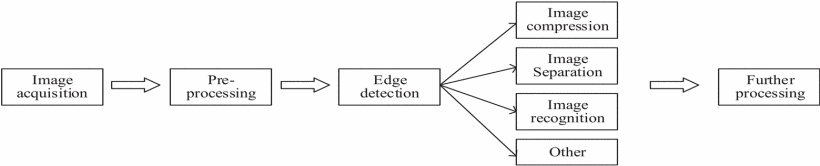
\includegraphics[width=1\textwidth]{Pipeline.png}
    \caption{Pipeline for image analysis techniques \cite{RTEdge}}
    \label{fig:pipeline}
\end{figure}

\cite{SoCImage, Aerial} follow a similar pipeline to Figure \ref{fig:pipeline}, with the image being captured by a camera module, and then processed by an FPGA though using differing image techniques.
These found that FPGAs can accelerate the required multiplication and addition operators separately - required for classical, and deep learning, based techniques \cite{ResourceEfficient}.
By leveraging the parallel processing capabilities of FPGAs to handle the convolution operations, the techniques can be accelerated to provide real-time image processing capabilities.

\section{Convolution}
Convolution operations form the computational foundation of many image processing and neural network applications.
It is referred to as a Single Instruction Multiple Data (SIMD) operation, as it performs the same operation on multiple data points in parallel \cite{7}.
In CNNs, convolution layers typically consume over 99\% of the total computational and storage resources \cite{18}.
Other sources estimate that convolution accounts for 90\% of the total execution time of CNNs, with between 50 to 90\% of the total operations being convolution \cite{3, 2}.
The operation involves sliding a kernel across input data, performing multiply-accumulate (MAC) operations between the kernel values and the input values at each position \cite{7}.
This process is depicted in Figure \ref{fig:convolution}.

\begin{figure}[h]
    \centering
    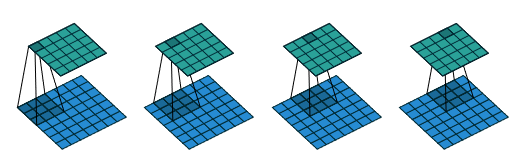
\includegraphics[width=1\textwidth]{Convolution.png}
    \caption{Convolution utilising a 3x3 kernel \cite{19}}
    \label{fig:convolution}
\end{figure}

For a single output pixel using an \(m \times n\) convolution mask, \(m \times n\) multiplications and \(m \times n-1\) additions are required. 
This computational intensity is demonstrated by the fact that processing a modest \(256 \times 256\) grayscale image with a \(3 \times 3\) mask requires \(589,824\) multiplications and \(65,535\) additions \cite{7}. 
The operation becomes even more resource-intensive when processing real-time video streams or larger images.
Hence, the convolution operation requires a large number of multiply-accumulate (MAC) operations, and is the primary bottleneck in the performance of CNNs \cite{11}.
The operation must window over the entire image, and the number of MAC operations is proportional to the size of the image and the number of filters in the layer.

Hardware implementations of convolution typically utilize one of two main approaches \cite{1}:
\begin{itemize}
    \item Direct computation using parallel processing units
    \item Data transformation methods, commonly used in frameworks like PyTorch and TensorFlow
\end{itemize}

FPGA implementations can significantly accelerate convolution operations through parallel processing. 
A common architecture involves storing image data and weights in block RAM (BRAM) \cite{7} or by embedding them in the FPGA fabric \cite{20} and implementing a finite state machine (FSM) to control pixel access and computation flow. 
Modern implementations often employ double-buffering techniques, where one buffer stores the working data while another handles intermediate results, enabling efficient pipelining of operations \cite{14}.

The pooling operation, which often follows convolution, operates similarly by sliding a window across the input but replaces the linear combination with alternative functions such as maximum or average calculations \cite{19}. 
Hence, it similarly shares the same hardware resources for adders and multipliers to compute.
This helps reduce the spatial dimensions of the data while retaining important features.

The number of operations, or hardware resources, required for convolution can be reduced through a number of optimization techniques. 
\begin{itemize}
    \item Quantisation to reduce precision requirements \cite{12}
    \item Sparsification to eliminate unused weights \cite{11}
    \item Time-division multiplexing (folding) of computing resources \cite{14}
    \item Streaming architectures that enable layer pipelining \cite{16}
\end{itemize}

These optimizations are particularly important for embedded systems and edge devices where computational resources and power consumption are constrained. 
For instance, quantization can reduce precision from 32-bit floating-point to 8-bit integer representations while maintaining accuracy within 0.1\% \cite{12}.
Other techniques can be used to compress the parameters to reduce the memory requirements \cite{18}.

\section{Convolutional Neural Networks}
Convolutional neural networks (CNNs) are a type of artificial neural network that is primarily used for image detection, as it uses the convolution kernel to detect features in the image.
Due to the lack of memory in low-end FPGA models, the CNN is optimal for an image processing task on SoC, as it has a low number of weights and biases relative to other neural networks \cite{Drowsiness}.
This makes it viable to implement machine learning cores through a CNN using on-board resources with some optimisations compared to other more storage-intensive networks \cite{14}.

Similar works for image-analysis using different neural network architectures have also been implemented using FPGA hardware.
\cite{Yolo, SparseYolo} demonstrates a hardware implementation of the You Only Look Once (YOLO) algorithm using a Xilinx Virtex-7 FPGA. 
Like the CNN hardware implementations, the architecture is focused on accelerating the convolution operation - and is a common denominator in the performance neural networks in hardware.
This acceleration is not specific to the convolution operator, and can be applied to any intensive operation in the network as the FPGA has little overhead on each operator when compared to traditional platforms \cite{Overhead}.
This is corroborated by \cite{Throughput}, which found that the implementation of hybrid neural networks on a Xilinix Virtex-7 690T FPGA achieved 4.13 times higher throughput than state of the art accelerators in 2019.


\section{RISC-V}
Instruction set architectures (ISAs) define the operations a processor can execute, however, the majority of ISAs are proprietary and require licensing to use.
Reduced Instruction Set Computing (RISC) is a form of ISA which offers a simpler, more efficient design than the traditional Complex Instruction Set Computing (CISC) ISAs - such as the prevalent x86 instruction set \cite{Arm}.
Arm and RISC-V are the two most prominent RISC ISAs, with Arm being the most widely used in embedded systems but with RISC-V offering royalty-free licensing and an open-source nature.
The lack of licensing fees and the open-source nature of RISC-V has led to its increasing popularity in the embedded systems domain \cite{Neutron}.
It is estimated that the number of chips utilising RISC-V technology "will grow 73.6 percent per year to 2027, when there will be some 25 billion AI chips produced, accounting for US \$291 billion in revenue" \cite{Drowsiness}.


There exists a number of FPGA implementations to create softcore processors using the RISC-V ISA \cite{RISCFPGA}. 
This 2023 paper \cite{Neutron} demonstrates a RISC-V implementation of the NEORV32 core, using a Wishbone bus interface. 
The authors selected the NEORV32 core due to it being vendor-agnostic and platform independent, with the project being highly documented.
The softcore nature allows for the implementation details to be customised to the specific application, such that the core can be adapted to the specific use case \cite{DCT}. 
The NEORV32 processors offers a system-on-chip (SoC) Harvard architecture, with a 32-bit RISC-V processor, and a range of peripherals.
It supports UART, SPI, standard GPIO and the Wishbone b4 external bus interface for SoC connectivity \cite{NEORV32}.

As it is an open-source ISA, RISC-V has the added benefit of being extensible and modular \cite{Cryptography}, allowing for instructions to be added to the processor.
\cite{Reconfigurable} utilises this to create custom instructions within the RISC-V ISA to accelerate the expensive convolution operation for a CNN.
Other applications have also extended the architecture to include custom instructions for frequently used and computationally-expensive operations.

\section{Computing Platforms}
\label{sec:platforms}
The nature of convolution, and many of the layers in CNNs, benefit significantly from parallel processing capabilities.

Field Programmable Gate Arrays (FPGAs) provide flexible compute resources that can be reconfigured to suit a wide range of applications. Similar to graphics processing units (GPUs), FPGAs offer parallel processing capabilities, but with the added benefit of reconfigurability \cite{Parallelism}. The ability to develop custom logic designs is not unique to FPGAs, as application-specific integrated circuits (ASICs) also offer this capability. ASICs offer better optimization in many aspects than FPGAs, but cannot be reconfigured and require a large upfront cost for design and fabrication \cite{AsicOptimization}. This makes FPGAs a more suitable platform for low-volume production and prototyping, as they offer a faster development cycle and lower cost than ASICs.

In contrast, traditional Central Processing Units (CPUs) are designed for serial processing, executing a single instruction stream at a time - see figure \ref{fig:cpu_gpu}. This architecture is optimized for low-latency tasks and complex control logic, making CPUs highly effective for general-purpose computing. However, their performance can be limited when handling tasks that require high levels of parallelism, such as those found in image processing and deep learning applications. 
On the other hand, GPUs are specifically designed for parallel processing, featuring thousands of cores that can execute multiple threads simultaneously. 
This architecture allows GPUs to handle large datasets and perform computations in parallel, significantly speeding up tasks like matrix multiplications and convolutions, which are fundamental in CNNs \cite{15}.
The parallel architecture can be implemented in FPGA fabric, to achieve drastic speedups.
\cite{10} demonstrates a twenty-times speedup of the throughput when the network was compared to a CPU implementation, similar or better results would be expected for a GPU implementation.

The CUDA (Compute Unified Device Architecture) platform, developed by NVIDIA, further enhances the capabilities of GPUs by providing a parallel computing framework that allows developers to leverage the power of GPU cores, known as CUDA cores. Each CUDA core is capable of executing a thread, and with thousands of these cores available, GPUs can perform massive parallel computations efficiently \cite{4}. This makes CUDA particularly well-suited for applications in machine learning, where the ability to process large amounts of data simultaneously is crucial \cite{22}. 

NVIDIA's GPUs are designed with a focus on high throughput and efficiency, making them ideal for tasks that require extensive computational power. The architecture of NVIDIA GPUs includes multiple Streaming Multiprocessors (SMs), each containing several CUDA cores \cite{4}. This design allows for the simultaneous execution of thousands of threads, enabling the GPU to handle complex calculations much faster than a CPU. For instance, while a CPU may have a few cores optimized for sequential processing, a modern NVIDIA GPU can have thousands of CUDA cores working in parallel, which is particularly beneficial for deep learning tasks that involve large matrices and tensors.

The combination of GPU architecture and the CUDA platform has led to significant advancements in the performance of deep learning algorithms, enabling real-time processing and analysis of complex datasets. 
For example, in image recognition tasks, the parallel processing capabilities of GPUs allow for the rapid analysis of thousands of images simultaneously, which is essential for training deep neural networks effectively \cite{16}.

These reconfigurable platforms are optimal for edge applications on images, due to the parallelized pipeline structure, which enables high-speed processing of large amounts of image data, and their high processing speed ensures real-time image data processing \cite{Video}. FPGAs in particular have been studied extensively in the field of image detection, as replacements for existing hardware infrastructures due to the increasing complexity of algorithms \cite{ResearchFPGA}. They offer low latency and low power consumption due to their computing characteristics. However, the ability to configure often means that resource constraints and utilization must be considered when designing the system, such as with many embedded devices.

\begin{figure}[h]
    \centering
    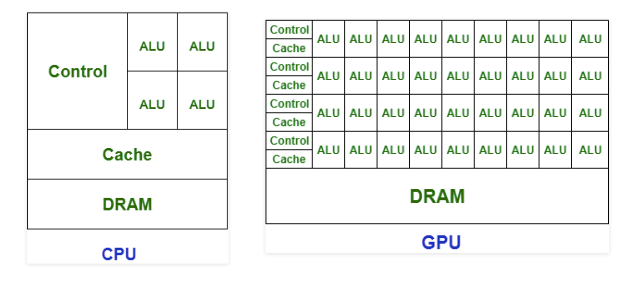
\includegraphics[width=0.8\textwidth]{cpu.png}
    \caption{Comparison of logic units between CPU and GPU \cite{21}}
    \label{fig:cpu_gpu}
\end{figure}

%CHAPTER 3

% ***************************************************
% Example of an internal chapter
% ***************************************************
%This is an internal chapter of the thesis.
%If you have a long title, you can supply an abbreviated version to print in the Table of Contents using the optional argument to the \chapter command.
\chapter[Design]{Design}
\label{chap:Design}	%CREATE YOUR OWN LABEL.
\pagestyle{headings}

This chapter justifies the design choices for implementing a convolutional core at a hardware level, and associated hardware configuration.
As per the aims, it primarily focuses on a robust framework for convolution and secondary a means to extend this to a convolutional neural network.

\section{Hardware Implementation}
\subsection{FPGA}
The project employs a Digilent Basys 3 Artix-7 FPGA development board (figure \ref{fig:dev_board}).
This is an introductory model, and hence is very resource limited - enabling for the demonstration of hardware accelerators for constrained devices.
The FPGA is of the Artix-7 family, and is optimised for low power designs with high logic throughput \cite{Xilinx7SeriesDatasheet}. 
The model used is the XC7A35T-1CPG236C, which has 33280 logic cells, 1,800Kbits of fast block RAM (BRAM) and internal clock speeds exceeding 450MHz \cite{basys}.
The clock will be limited to 100MHz for the purposes of this project, to ensure route and place is successful.

No external memory is supported, and as such the hardware will be limited to only the on-board resources.

\begin{figure}[h!]
    \centering
    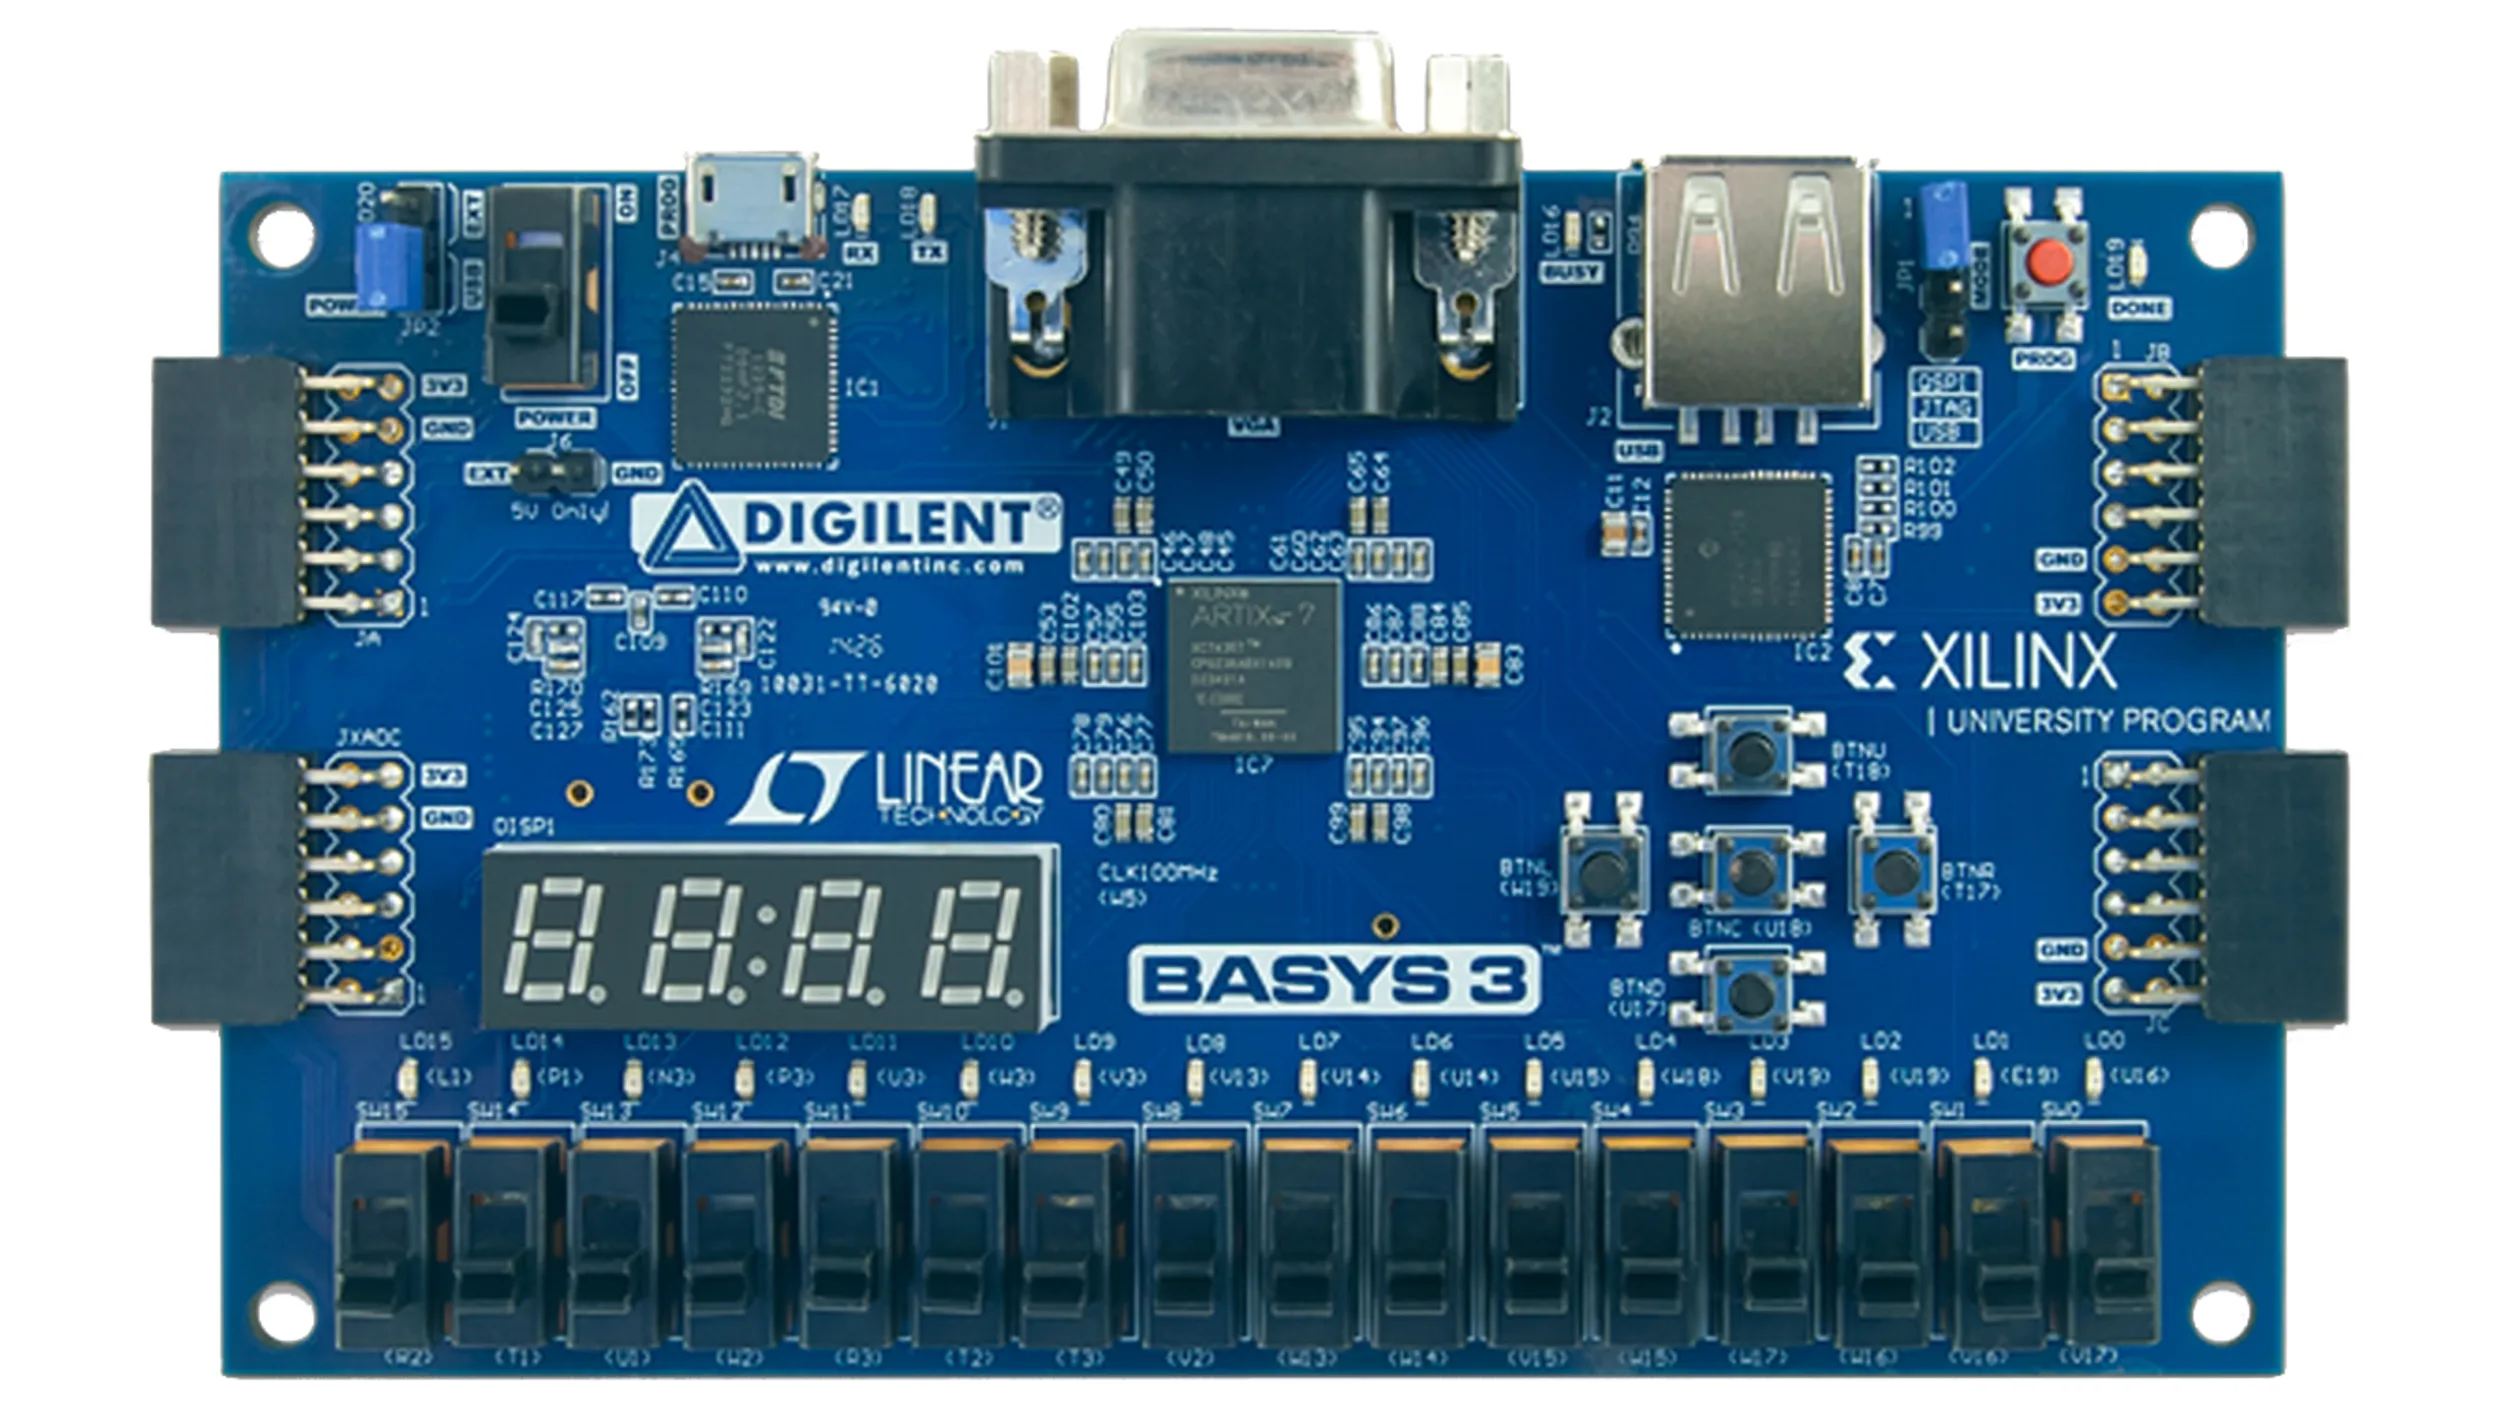
\includegraphics[width=0.65\textwidth]{basys3.png}
    \caption[Digilent Basys 3 FPGA development board]{Digilent Basys 3 FPGA development board.}
    \label{fig:dev_board}
\end{figure}

\newpage


\subsection{RISC-V Softcore}

FPGAs provide full configurability of the hardware, and offer softcore processors as a means to control the hardware.
A system on chip (SoC) is implemented on the FPGA, and is controlled by a RISC-V softcore processor which provides a method to control the hardware and run higher layer tasks, which is generally required for embedded systems being simulated here.
Fundamentally, it provides a mapping to pass data to the dedicated hardware and access the signals to retrieve the results.

The NeoRV32 softcore implementation was selected due to it's highly documented ecosystem, and personal familiarity\footnote[1]{See: https://github.com/stnolting/neorv32}.
For connecting the processor to the FPGA, the Wishbone B4 classic bus was selected due to it's high bandwidth and relatively easy implementation - as the NeoRV32 natively supports the interface.
The bus uses a 32-bit data width, as the primary use is to allow for mapping of a memory address for the accelerator to retrieve the image data from.

\subsection{Convolution}
\label{sec:convolution}

Convolution operations form the computational foundation of modern image processing algorithms and neural networks, transforming input data into higher-dimensional feature representations. In Convolutional Neural Networks (CNNs), these operations constitute approximately 90% of the total computational workload during inference [citation needed], making them the primary bottleneck in system performance.

The mathematical formulation of a 2D convolution with multiple input channels can be expressed as:

\begin{equation}
    Y(i,j) = \sum_{m=0}^{K-1} \sum_{n=0}^{K-1} \sum_{c=0}^{C-1} X(i+m,j+n,c) \cdot W(m,n,c)
\end{equation}

where $X$ represents the input feature map, $W$ represents the convolution kernel, $K$ denotes the kernel size, $C$ represents the number of input channels, and $Y$ is the resulting output feature map.

Hardware acceleration of convolution operations offers several critical advantages:

\begin{itemize}
    \item \textbf{Computational Offloading}: Dedicated FPGA hardware handles intensive convolution computations, freeing the main processor for other critical tasks
    \item \textbf{Parallel Processing}: The inherent parallelism of FPGA architectures enables concurrent execution of multiple convolution operations
    \item \textbf{Deterministic Performance}: Hardware implementation ensures consistent execution times, crucial for real-time applications
    \item \textbf{Energy Efficiency}: Dedicated hardware structures provide better performance-per-watt compared to general-purpose processors
\end{itemize}

The convolution accelerator is implemented using parameterizable hardware description language (HDL) generics, enabling compile-time optimization. This approach eliminates runtime initialization overhead and allows for application-specific tailoring. Table \ref{tab:convolution_parameters} details the key parameters governing the convolution operation for this implementation.

\begin{table}[h!]
    \centering
    \caption{Key parameters for hardware convolution implementation}
    \label{tab:convolution_parameters}
    \begin{tabular}{ccc}
        \toprule
        Parameter & Symbol & Description \\
        \midrule
        Image Size & I & Input feature map dimensions (height × width) \\
        Kernel Size & K & Convolution kernel dimensions (K × K) \\
        Input Channels & C & Number of input feature map channels \\
        Bit Width & Q & Fixed-point precision for values \\
        Output Channels & O & Number of output feature maps \\
        Stride & S & Convolution window step size \\
        Zero Padding & Z & Padding width applied to input boundaries \\
        \bottomrule
    \end{tabular}
\end{table}

The hardware architecture employs a custom type system to abstract multi-dimensional data structures. Feature maps, which represent either input images or intermediate representations, are modeled as three-dimensional matrices of pixels (height × width × channels). This abstraction is implemented through a parameterized array type that can be efficiently mapped to hardware vectors.

At the implementation level, these higher-dimensional structures are flattened into single-dimensional vectors, with careful attention to maintaining spatial relationships. This approach provides several advantages:

\begin{itemize}
    \item \textbf{Memory Efficiency}: Optimized storage and access patterns for FPGA block RAM
    \item \textbf{Hardware Mapping}: Direct correspondence between logical and physical data organization
    \item \textbf{Abstraction}: High-level interface for design and verification while maintaining low-level efficiency
\end{itemize}

\subsubsection{MAC Unit}

The Multiply-Accumulate (MAC) unit forms the fundamental computational element of the convolution operation in hardware. Each MAC unit comprises dedicated DSP blocks or equivalent arithmetic units for multiplication and cascaded adder trees for accumulation, optimized for the FPGA fabric.

The basic MAC operation for a single convolution point can be expressed as:

\begin{equation}
    y = \sum_{i=0}^{n} w_i \cdot x_i
\end{equation}

where $w_i$ represents kernel weights and $x_i$ represents input feature values.

\begin{figure}[h]
    \centering
    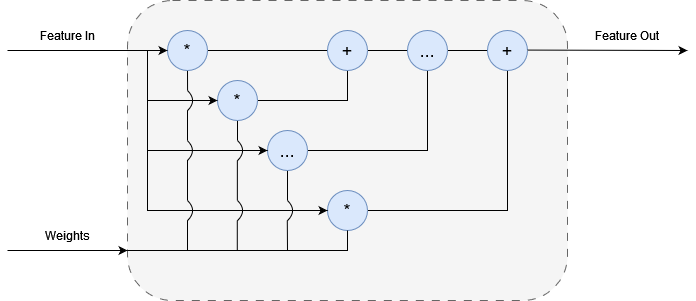
\includegraphics[width=0.75\textwidth]{mac.png}
    \caption{Hardware architecture of the MAC unit showing parallel multipliers and adder tree configuration.}
    \label{fig:mac}
\end{figure}

Resource utilization scales with the kernel dimensions according to:
\begin{equation}
    \text{DSP}_{\text{total}} = K \times K \times C
\end{equation}

where $K$ is the kernel size and $C$ is the number of input channels. 

The MAC units operate on fixed-point arithmetic to maintain precision while optimizing hardware resources, with parameterizable bit widths allowing for application-specific trade-offs between precision and resource utilization.
However, as the size of the feature map and kernel increases, the number of MAC units required increases proportionally to the kernel size.
To reduce the number of MAC units required, the concept of folding is introduced.
This is a method to reduce the number of MAC units required by sharing the MAC units across time.
This is achieved by partitioning the input data into slices which can then be pipelined through the MAC units, and as such the resources are shared across different time intervals to reduce the amount of resources required.
The following sections detail the implementation of folding for convolution to reduce the required resources.

\clearpage 
\subsubsection{No Folding}

Convolution without folding is a fully parallelised approach, whereby the entire kernel is moved across the image in a single clock cycle.
This is naturally implicit for hardware description languages, as operations are inherently performed in parallel (see listing \ref{lst:code_snippet}).

\begin{lstlisting}[style=vhdl, caption={Implementation of fully parallelised convolution}, label=lst:code_snippet]
for conv_row in feature_o'range(1) loop
    for conv_col in feature_o'range(2) loop
        for conv_chan in feature_o'range(3) loop            
            for mac_row in weights_i'range(1) loop
                for mac_col in weights_i'range(2) loop
                    for mac_chan in 1 to C loop
                        ----- ... -----
                    end loop;
                end loop;
            end loop;
        end loop;
    end loop;
end loop;
\end{lstlisting}

The operation will then be dependent on the fastest clock speed possible for the FPGA to ensure the timing constraints are met, as the additions must complete within the clock cycle.
It utilises the described MAC units in figure \ref{fig:mac} for each slice of an image, with the corresponding kernel weight slice.
This is represented by the feature map type, which represents the slicing of the image matrix.
Zero padding is applied as necessary based on the design generics at the tail and head of the image matrix, in each dimension.
The convolution process in hardware is described in figure \ref{fig:conv}.



\begin{figure}[h]
    \centering
    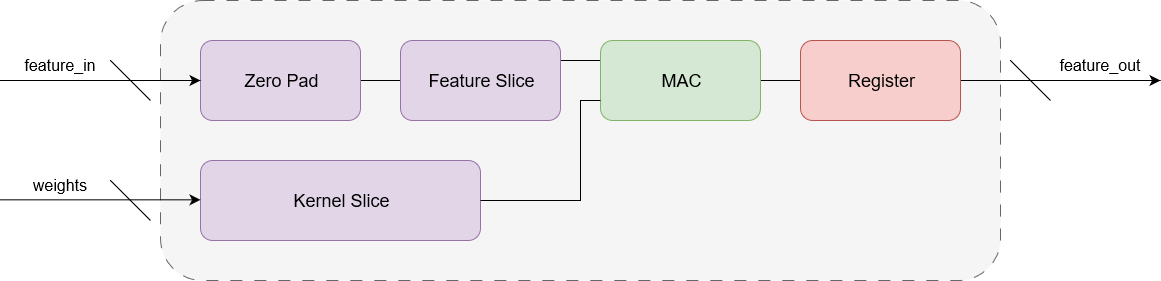
\includegraphics[width=0.75\textwidth]{conv.png}
    \caption{Convolution operation without folding.}
    \label{fig:conv}
\end{figure}


\subsubsection{Partial Folding}
A partially folded approach improves the sustainability of implementing a kernel with concern for the available hardware resources.
This is achieved by migrating to a partial dataflow approach, where the MAC units are shared across the kernel size.
It implements time multiplexing to remove the need for additional MACs based on the desired output channels.

To achieve this, an iterator is implemented to step through the values contained in the feature map and corresponding kernel weights, shown in figure \ref{fig:iterator}.
This produces a smaller slice of the image which is passed to the MAC units for processing.
It is then demultiplexed to produce the final result back as the feature map type.
This approach requires a small amount of extra logic to handle the partial slices, however, it has a marked decrease in the required resources, and as such is a more sustainable approach.

\begin{figure}[h]
    \centering
    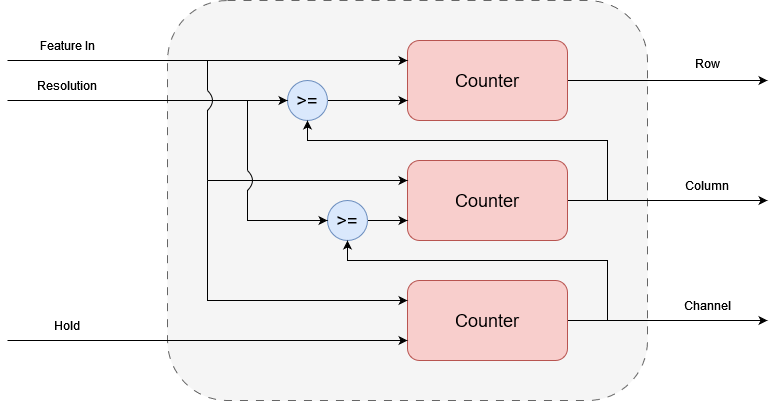
\includegraphics[width=0.75\textwidth]{iterator.png}
    \caption{Hardware representation of the MAC unit.}
    \label{fig:iterator}
\end{figure}

The fully parallelised approach can be modified to include folding by utilising the iterator to step through the feature map and kernel weights.
This is shown in figure \ref{fig:partial_folded}.

\begin{figure}[h]
    \centering
    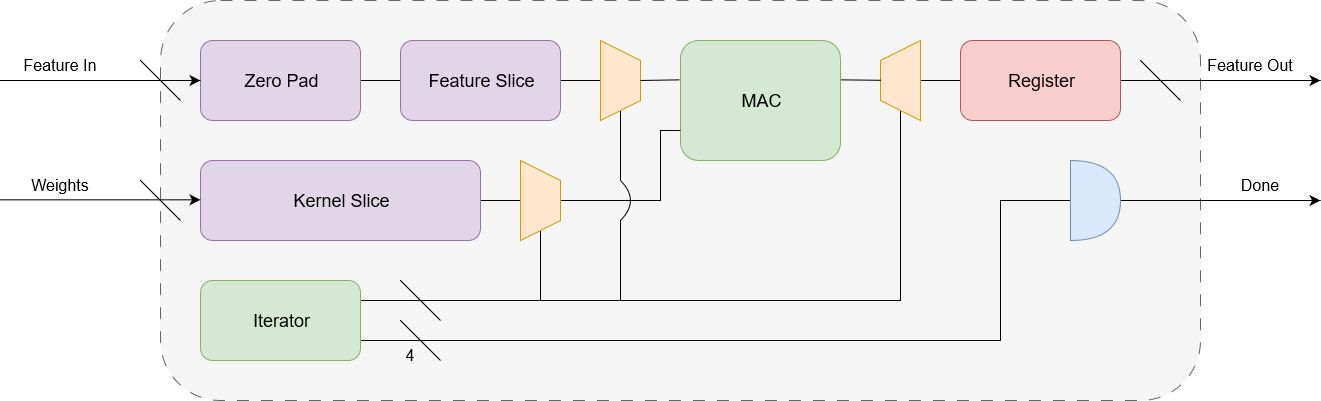
\includegraphics[width=0.75\textwidth]{conv_partially_folded.png}
    \caption{Convolution operation with partial folding via the iterator.}
    \label{fig:partial_folded}
\end{figure}



\subsubsection{Complete Folding}
A complete folding approach involves a single MAC unit that is shared across the entire image.
This will introduce a constant number of MAC units, agnostic to the kernel size.
However, the tradeoff comes at additional logic to handle the iteration of the feature map and kernel weights.

To implement the slicing of individual feature map values and kernel weights, a complete dataflow architecture is implemented.
This requires a transmit module to handle the slicing of the feature map, and a receive module to handle the slicing of the kernel weights.
These form the control unit in the form of a finite state machine to coordinate the streaming of data to the MAC unit.
As convolution requires the summation of a number of values, the receive module must store the partial results until all the values have been summed to produce the final result when the iteration is complete.
This is shown in figure \ref{fig:fully_folded}.

\begin{figure}[h]
    \centering
    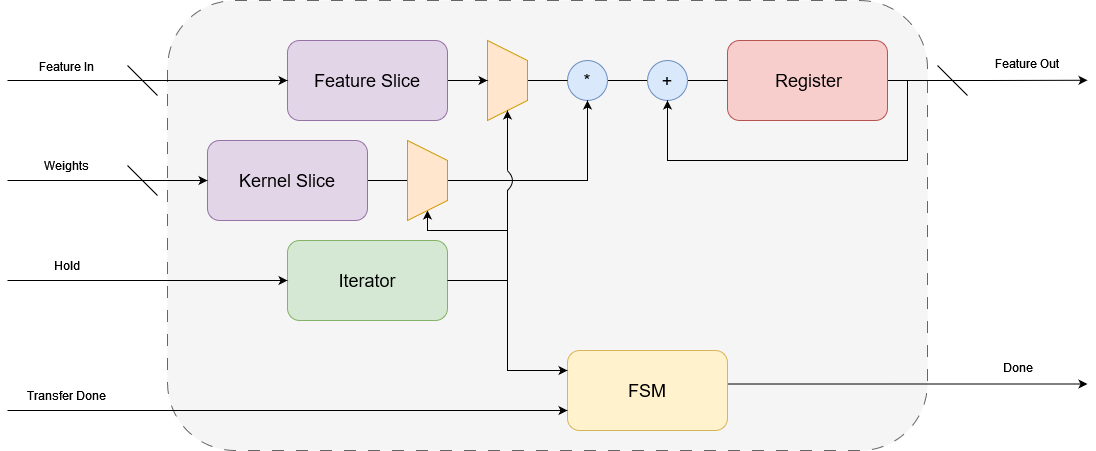
\includegraphics[width=0.75\textwidth]{fully_folded_conv.png}
    \caption{Hardware representation of the MAC unit.}
    \label{fig:fully_folded}
\end{figure}

\subsection{Activation Function}
The activation function is used to introduce non-linearity to the model, which fundamentally enables it to model complex patterns and relationships in data \cite{DCNN}. The most common activation function used in CNNs is the Rectified Linear Unit (ReLU), which is defined as:
\label{sec:relu}

\begin{equation}
    f(x) = \max(0, x)
\end{equation}

This was selected over other activation functions such as the Sigmoid and Tanh due to its computational efficiency and ease of implementation at a hardware layer \cite{10}. The hardware implementation consists of a comparator and multiplexer to select between zero and the input value, as shown in figure \ref{fig:relu}.

\begin{figure}[h]
    \centering
    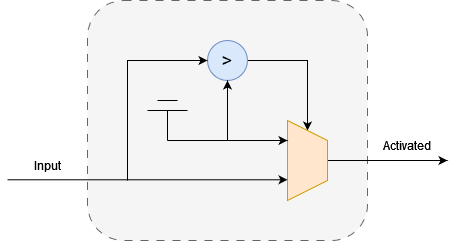
\includegraphics[width=0.65\textwidth]{relu.png}
    \caption{Hardware implementation of ReLU activation function}
    \label{fig:relu}
\end{figure}

While activation functions could be implemented as standalone modules, the ReLU implementation is integrated directly into the convolution module for several key reasons:

\begin{itemize}
    \item \textbf{Timing Efficiency}: The activation can be performed within the same clock cycle as the final MAC operation, eliminating additional pipeline stages \cite{14}
    \item \textbf{Resource Optimization}: Integration allows sharing of control signals and timing logic, reducing overall resource utilization
    \item \textbf{Reduced Complexity}: Direct integration eliminates the need for additional interface logic and buffering between modules
\end{itemize}

The hardware implementation leverages the fact that negative numbers in two's complement representation have their most significant bit (MSB) set to 1. Therefore, the comparator only needs to examine this bit to determine if the input is negative, making the implementation particularly efficient in terms of both latency and resource utilization. The multiplexer then selects either zero or the input value based on this single-bit comparison.

This architectural decision follows established principles of hardware optimization, where tightly coupled operations are combined to minimize both latency and resource usage. The marginal increase in convolution module complexity (approximately 32 LUTs per output channel) is justified by the benefits of reduced latency and simplified control logic, particularly important for resource-constrained FPGA implementations \cite{16}.

\subsection{Pooling Layer}
\label{sec:pooling}

Pooling layers are used to reduce the spatial dimensions of the feature maps while retaining important information \cite{19}. The max pooling operation is implemented using a sliding window approach, similar to convolution, but instead of multiplication and accumulation, it performs a comparison operation between values.

At a hardware level, each pooling unit consists of a comparator that determines the maximum value between two inputs. This is significantly more resource-efficient than MAC units as it only requires comparison logic. For a 2x2 pooling window with stride 2, the output dimensions are halved in both spatial dimensions, effectively reducing the computational complexity of subsequent layers \cite{10}.

The hardware implementation can be approached in two ways:
\begin{itemize}
    \item \textbf{Parallel Implementation}: All comparisons within a pooling window are performed simultaneously, requiring multiple comparator units but providing single-cycle operation
    \item \textbf{Folded Implementation}: A single comparator is time-multiplexed across the pooling window, reducing resource utilization at the cost of increased latency
\end{itemize}

As shown in figure \ref{fig:pooling_hardware}, the design implements a parallel approach for the 2x2 pooling window. This decision was made because:
\begin{itemize}
    \item The resource cost of comparators is significantly lower than MAC units
    \item Parallel implementation maintains the dataflow of the convolution output
    \item The reduced feature map size already provides significant computational savings
\end{itemize}

\begin{figure}[h]
    \centering
    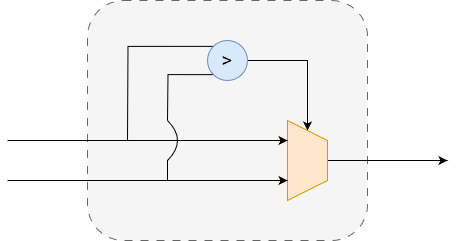
\includegraphics[width=0.75\textwidth]{pool.png}
    \caption{Hardware implementation of max pooling layer showing parallel comparator arrangement}
    \label{fig:pooling_hardware}
\end{figure}

The pooling operation can be expressed mathematically as:

\begin{equation}
    y_{i,j} = \max_{m,n \in R} x_{i+m,j+n}
\end{equation}

where $R$ represents the pooling region (2x2 in this implementation), and $(i,j)$ are the output coordinates. This operation requires significantly fewer resources than convolution while providing essential dimensionality reduction for the neural network architecture \cite{18}.

\subsection{Fully Connected Layer}
\label{sec:fully_connected}

The fully connected layer performs a matrix multiplication between the input features and the weight matrix. This operation can be decomposed into a series of dot products, which can be implemented using MAC units similar to those used in the convolution layer \cite{ResourceEfficient}. The primary difference is that fully connected layers operate on flattened 1D vectors rather than 2D feature maps.

The hardware implementation utilizes parallel MAC units to compute multiple dot products simultaneously. The number of parallel units can be configured based on available resources and desired throughput. For a layer with $N$ inputs and $M$ outputs, the operation can be expressed as:

\begin{equation}
    y_j = \sum_{i=1}^{N} w_{ij}x_i + b_j
\end{equation}

where $y_j$ is the $j$th output, $w_{ij}$ represents the weight connecting input $i$ to output $j$, $x_i$ is the $i$th input, and $b_j$ is the bias term.

Similar to the convolution layer, the fully connected layer can be implemented with different levels of folding. However, this is not explored in this implementation as it is a specific to neural network architectures and not general image processing.
It is mentioned here for completeness.

\begin{itemize}
    \item \textbf{No Folding}: Requires $N \times M$ MAC units, providing maximum throughput but highest resource utilization
    \item \textbf{Input Folding}: Time-multiplexes the input vector, requiring $M$ MAC units
    \item \textbf{Complete Folding}: Uses a single MAC unit iteratively, minimizing resource usage at the cost of increased latency
\end{itemize}

For the implemented design, input folding was selected as it provides a reasonable compromise between resource utilization and performance \cite{16}. This approach:
\begin{itemize}
    \item Reduces hardware complexity compared to full parallelization
    \item Maintains acceptable throughput for inference operations
    \item Allows for efficient resource sharing with convolution layers
    \item Simplifies control logic and data routing
\end{itemize}

The timing characteristics of the folded implementation can be determined by:

\begin{equation}
    \text{Cycles} = N + P
\end{equation}

where $N$ is the number of inputs and $P$ is the pipeline depth of the MAC unit. This demonstrates how the latency scales linearly with input size, making it suitable for resource-constrained FPGA implementations \cite{17}.

\section{Network Quantization}
\label{sec:quantization}

Quantization is essential for efficient hardware implementation of neural networks.
It reduces memory requirements and simplifies computations by converting floating-point values to fixed-point or integer representations.
The process must be carefully managed to maintain model accuracy while reducing precision.

\subsection{Training-Aware Quantization}
\label{sec:training_quantization}

To maintain accuracy while reducing precision, quantization is performed during the training process.
This allows the network to adapt its weights to compensate for the reduced precision.
The quantization process is as follows:

\begin{enumerate}
    \item Define quantization parameters (bit width, scaling factors)
    \item Forward pass with quantized weights and activations
    \item Backward pass with straight-through estimator
    \item Update full-precision weights
    \item Quantize updated weights
\end{enumerate}

The quantization function Q(x) for an n-bit fixed-point representation is defined as:

\begin{equation}
    Q(x) = \text{round}(x \cdot 2^n) \cdot 2^{-n}
\end{equation}

For the design, the network is quantized in training to utilise an 8-bit integer representation.
This is effectively analogous to using a fixed-point representation, with the scaling factor being $2^8$, which is recommendation for future work to better generalise the layers developed.

\section{Neural Network Implementation}

\subsection{Dataset}
As part of the design, a dataset of images was required to demonstrate recognition capabilities of the accelerator built on top of the convolutional core.
Digit-based datasets, such as MNIST, are commonly used for demonstrating the capabilities of CNNs and are therefore used for this project.
The digit dataset used in this project consists of a down-sampled version of MNIST, with each image being 8x8 pixels in size using a single colour channel represented in 8-bit greyscale.
This is due to the resource limitations of the development board used, and to lower the time required for synthesis.
As the network is implemented at a hardware level, increasing the scale of the image is directly commensurate with the required resources and also training time.
A sample image of the dataset can be seen in figure \ref{fig:digit_dataset}.

\begin{figure}[h]
    \centering
    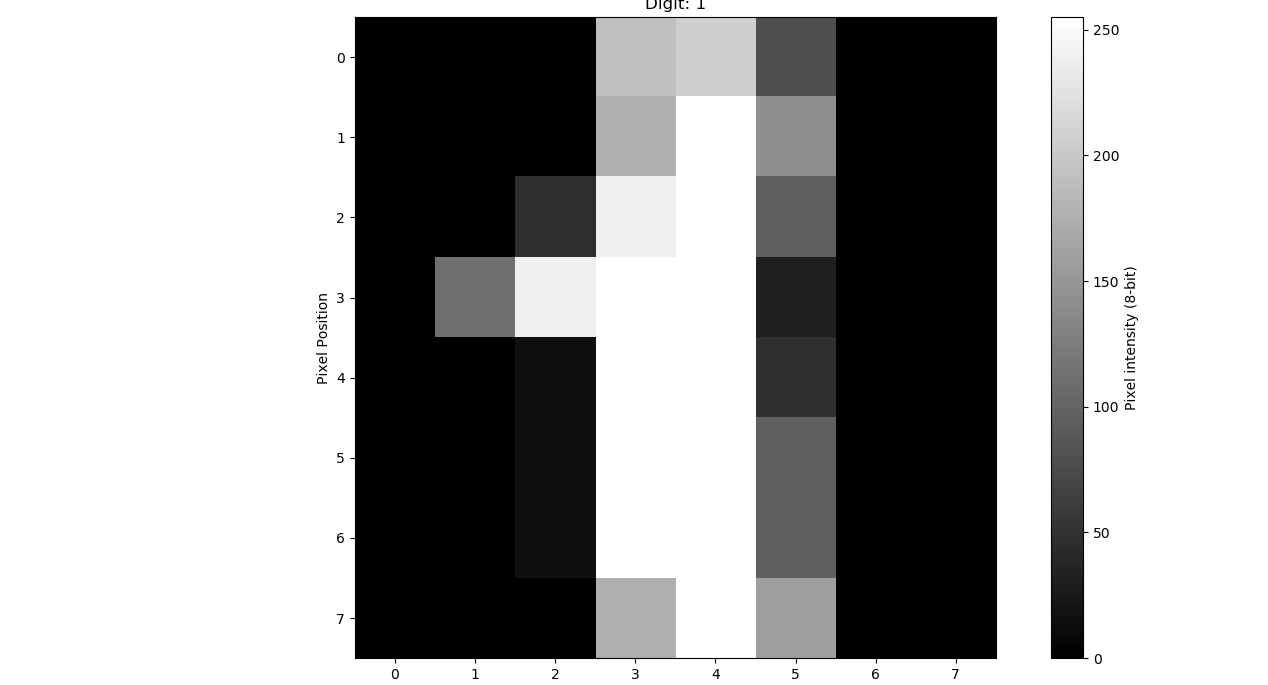
\includegraphics[width=0.5\textwidth]{digit.png}
    \caption{Sample images from the downsampled MNIST dataset used for training and inference}
    \label{fig:digit_dataset}
\end{figure}

\subsection{Model}
A convolutional neural network was trained in software with inference to be performed on the hardware accelerator.
The architecture selected is effectively the simplest possible CNN architecture to demonstrate the feasibility of the design.
It consists of a single convolutional layer, with a max pooling to downsample the data followed by a fully connected layer to classify the data.
The model description is shown in figure \ref{fig:model_architecture}.

\begin{figure}[h!]
    \centering
    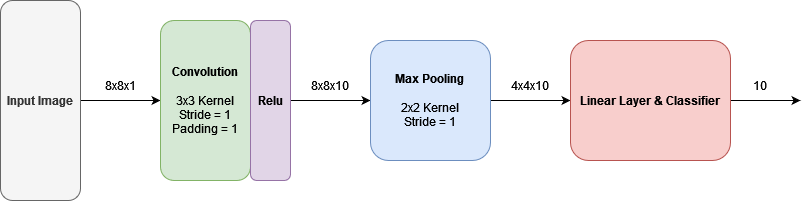
\includegraphics[width=0.65\textwidth]{model.png}
    \caption[Model architecture]{Model architecture.}
    \label{fig:model_architecture}
\end{figure}

The model was trained using an 80/20 split of the dataset, with 80\% used for training and 20\% used for validation.
The model was trained for 20 epochs with a batch size of 32.
As it is a classification problem, cross entropy loss was used as the loss function with an Adam optimiser to reduce the need for configuring learning rates.
It demonstrated an accuracy of 87\% on the validation set.
A summary of the network parameters can be seen in table \ref{tab:network_parameters}.
This is not discussed in detail as it is not central to the thesis, and is provided as reference for completeness.

\begin{table}[h!]
    \centering
    \caption{Summary of the network parameters.}
    \label{tab:network_parameters}
    \begin{tabular}{ccc}
        \toprule
        Parameter & Value & Description \\
        \midrule
        Loss function & Cross Entropy & Measure of accuracy \\
        Optimiser & Adam & Adaptive learning rate \\
        Batch Size & 32 & Number of samples per batch for training \\
        Epochs & 20 & Number of iterations to train the model \\
        Classes & 10 & Number of classes to classify as the output\\
        \bottomrule
    \end{tabular}
\end{table}

\subsection{Machine Learning Core}
The produced generic layers can be assembled to create a complete neural network, with a direct mapping from a software model.
There are two fundamental choices to be made when assembling the network:

\begin{enumerate}
    \item A streaming approach, where the next layer is loaded while the current layer is being processed
    \item A sequential approach, where each layer is processed in order
\end{enumerate}

Streaming architectures are typically more efficient in terms of resource utilisation, as they are non-blocking approaches.
The layers will have the outputs streamed to the following operation, while new input data is loaded into the current layer.
This fundamentally ensures that the layers are always fully utilised, and as such the resource utilisation of the design is minimised and can improve the latency.

A sequential approach is a single engine which executes the layers in order, and as such the resource utilisation is higher.
However, it is simpler to implement, and as such is more amenable to assembly from generic blocks.
It requires a single control block, via a FSM, to manage the dataflow between layers.
This makes it more extensible and flexible, but at the cost of increased resource utilisation and performance.
However, due to the simplicity of the design, it is the approach selected for this implementation.
This approach is shown in figure \ref{fig:ml_core}.

\begin{figure}[h]
    \centering
    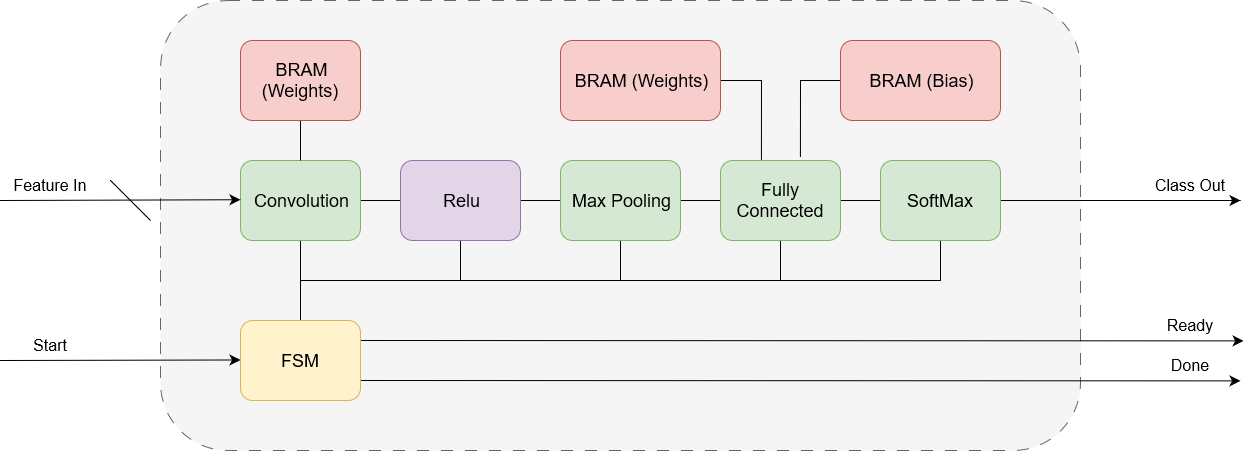
\includegraphics[width=0.75\textwidth]{ml_core.png}
    \caption{Hardware representation of the MAC unit.}
    \label{fig:ml_core}
\end{figure}

The machine learning core represents an assembly of the generic layers to form a complete neural network accessible via a memory mapped interface, using embedded network parameters at synthesis.
As discussed, a sequential architecture was selected due to the ability to implement virtually any network using the given components.
The core is controlled by a control unit, implemented as a finite state machine, to manage the dataflow between layers.
This is a relatively simple implementation, but provides a means to implement a wide range of networks with ease.


%CHAPTER 4

% ***************************************************
% Example of an internal chapter
% ***************************************************
%This is an internal chapter of the thesis.
%If you have a long title, you can supply an abbreviated version to print in the Table of Contents using the optional argument to the \chapter command.
\chapter[Results]{Results}
\label{chap:Results}	%CREATE YOUR OWN LABEL.
\pagestyle{headings}


The presented design provides a number of extensible blocks which can be configured to implement a simple convolutional neural network, or use the convolutional core to accelerate other image-processing algorithms. 
This chapter analyses the practicality of the design by assessing the throughput, resource utilisation and timing of the design.
The design is compared against CPU and GPU implementations to demonstrate the speedup to utilisation ratio, when compared to software-based implementations.

\section{Latency and Throughput}

Image processing algorithms are a prime candidate for hardware acceleration due to the large amount of data and the need for parallel processing.
This fundamentally makes reducing the latency of the design imperative, as outlined in section \ref{sec:convolution} - making this a critical metric for the design.
Latency is directly proportional to the number of clock cycles required to process the input image, and hence dictates the throughput of the design.

By developing the design at a hardware level, this allows for time deterministic performance, where the latency is known based on the convolution parameters.
The three designs presented in section \ref{sec:convolution} will require differing number of clock cycles, due to the varying levels of parallellisation to accomodate the varying FPGA resources.

\subsection{Time Determinism}
The advantage of an FPGA is the ability to implement the design at a hardware level, allowing for time deterministic performance.
As there are no overheads from the CPU or GPU, the latency is known based on the convolution parameters.
This allows for the latency to be determined at synthesis time, and the throughput to be calculated based on the number of clock cycles required to process the input image.

The fully parallel convolution implementation is constant, and will always require a single clock cycle to complete the operation \ref{eq:fully_parallel}.
\begin{equation}
    T_{fully\ parallel} = 1 \label{eq:fully_parallel}
\end{equation}

The partially folded implementation is dependent on the size of the kernel, and the stride. 
The image size is mutated by the size of the zero padding.
The defined variables can be found in table \ref{tab:convolution_parameters}.

\begin{equation}
    T_{partially\ folded} = \left( \frac{I + 2Z - K}{s} + 1 \right)^2 \times O
\end{equation}

The fully folded implementation is dependent on the same parameters, however, the kernel size is the primary driver for the number of clock cycles required.

\begin{equation}
    T_{fully\ folded} = K^2 \times C \times \left( \frac{I - K}{S} + 1 \right)^2 \times O
\end{equation}

\subsection{Implementation Timing}
The time deterministic nature of the FPGA allows for the timing of the design to be known at synthesis time.
This is in contrast to the CPU and GPU, where the timing is dependent on the computational workload and the underlying hardware.
Executing the design on an FPGA for the selected machine learning core parameters, the timing characteristics are as follows:

\begin{table}[h!]
    \centering
    \caption{Latency and throughput comparison of convolutional core implementations}
    \label{tab:latency_comparison}
    \begin{tabular}{lcccc}
        \toprule
        Implementation & Clock Cycles & Latency (ns) & Throughput (images/s) \\
        \midrule
        No Folding & 1 & 10 & 10e8 \\
        Partially Folded & 490 & 4900 & 2.04e5 \\
        Fully Folded & 1960 & 19600 & 5.1e4 \\
        \bottomrule
    \end{tabular}
\end{table}

There is a non-linear relationship between the level of folding and the latency of the design.
This is due to the increased number of MAC units required to process the input image, and the increased control logic required to manage the dataflow depending on the degree of folding.
The latency is computed based on the implementable design, where route and place succeeds - a clock speed of 100MHz is used for the FPGA.


\subsection{Comparison}
The performance characteristics of hardware-based convolution implementations can be evaluated against traditional computing platforms to understand their relative strengths and trade-offs. As discussed in section \ref{sec:platforms}, GPUs leverage thousands of CUDA cores for parallel processing, while CPUs rely on fewer but more complex processing units.

The NVIDIA Tesla P100 and A100 GPUs were selected as representative high-performance computing platforms, featuring dedicated hardware for parallel matrix operations. The P100 utilizes 3584 CUDA cores with 16GB of HBM2 memory, while the A100 represents NVIDIA's more recent architecture with 6912 CUDA cores and 40GB of memory (specifications detailed in \ref{app:device_information}). 
Relatively, the more modern A100 GPU provides is expected to provide an 11x speedup over the P100 - as shown in figure \ref{fig:nvidia}.
A standard Intel i7 CPU provides the baseline for comparison.

\begin{figure}[h]
    \centering
    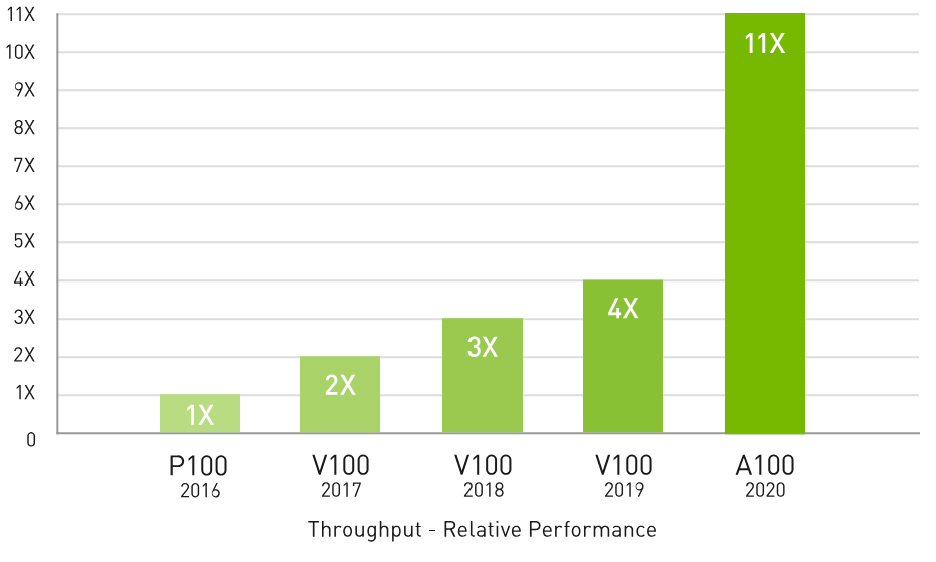
\includegraphics[width=0.75\textwidth]{nvidia.png}
    \caption{Comparison of relative performance of Nvidia GPUs \cite{23}.}
    \label{fig:nvidia}
\end{figure}

The performance comparison between implementations is presented in Table \ref{tab:platform_comparison}, which reveals several key insights:

\begin{itemize}
    \item The no-folding FPGA implementation achieves remarkable single-cycle latency (10ns), demonstrating the potential of fully parallel hardware implementations
    \item GPU implementations show strong performance, with the A100 achieving 609ns latency compared to the P100's 1020ns
    \item CPU implementation exhibits significantly higher latency at 229,782ns, highlighting the limitations of sequential processing
    \item The partially and fully folded FPGA implementations fall between CPU and GPU performance, with latencies of 4900ns and 19600ns respectively
\end{itemize}

This can be equally represented in terms of throughput, as shown in Table \ref{tab:latency_comparison}, as reducing the latency of convolution directly translates to an increase in throughput.
The throughput provides a more human-readable representation of the performance.

To provide context for these hardware implementations, Table \ref{tab:platform_comparison} compares their performance against traditional computing platforms:

\begin{table}[h!]
    \centering
    \caption{Platform comparison of latency and throughput}
    \label{tab:platform_comparison}
    \begin{tabular}{lcc}
        \toprule
        Device & Latency (ns) & Throughput (images/s) \\
        \midrule
        CPU (Intel i7) & 229782 & 4.35e3 \\
        Fully Folded & 19600 & 5.1e4 \\
        Partially Folded & 4900 & 2.04e5 \\
        Nvidia Tesla P100 GPU & 1020 & 9.8e6 \\
        Nvidia A100 GPU & 609 & 1.64e6 \\
        No Folding & 10 & 10e8 \\
        \bottomrule
    \end{tabular}
\end{table}

When considering throughput, the results demonstrate even more dramatic differences. 
The no-folding implementation theoretically achieves 10e8 images/s, though this is not practically achievable due to resource constraints. The GPU implementations demonstrate impressive real-world throughput, with the P100 processing 9.8e6 images/s and the A100 achieving 1.64e6 images/s. The CPU implementation manages only 4.35e3 images/s, while the partially folded and fully folded FPGA implementations achieve 2.04e5 and 5.1e4 images/s respectively.
The logarithmic scale of the throughput is provided in figure \ref{fig:throughput_comparison}.

\begin{figure}[h]
    \centering
    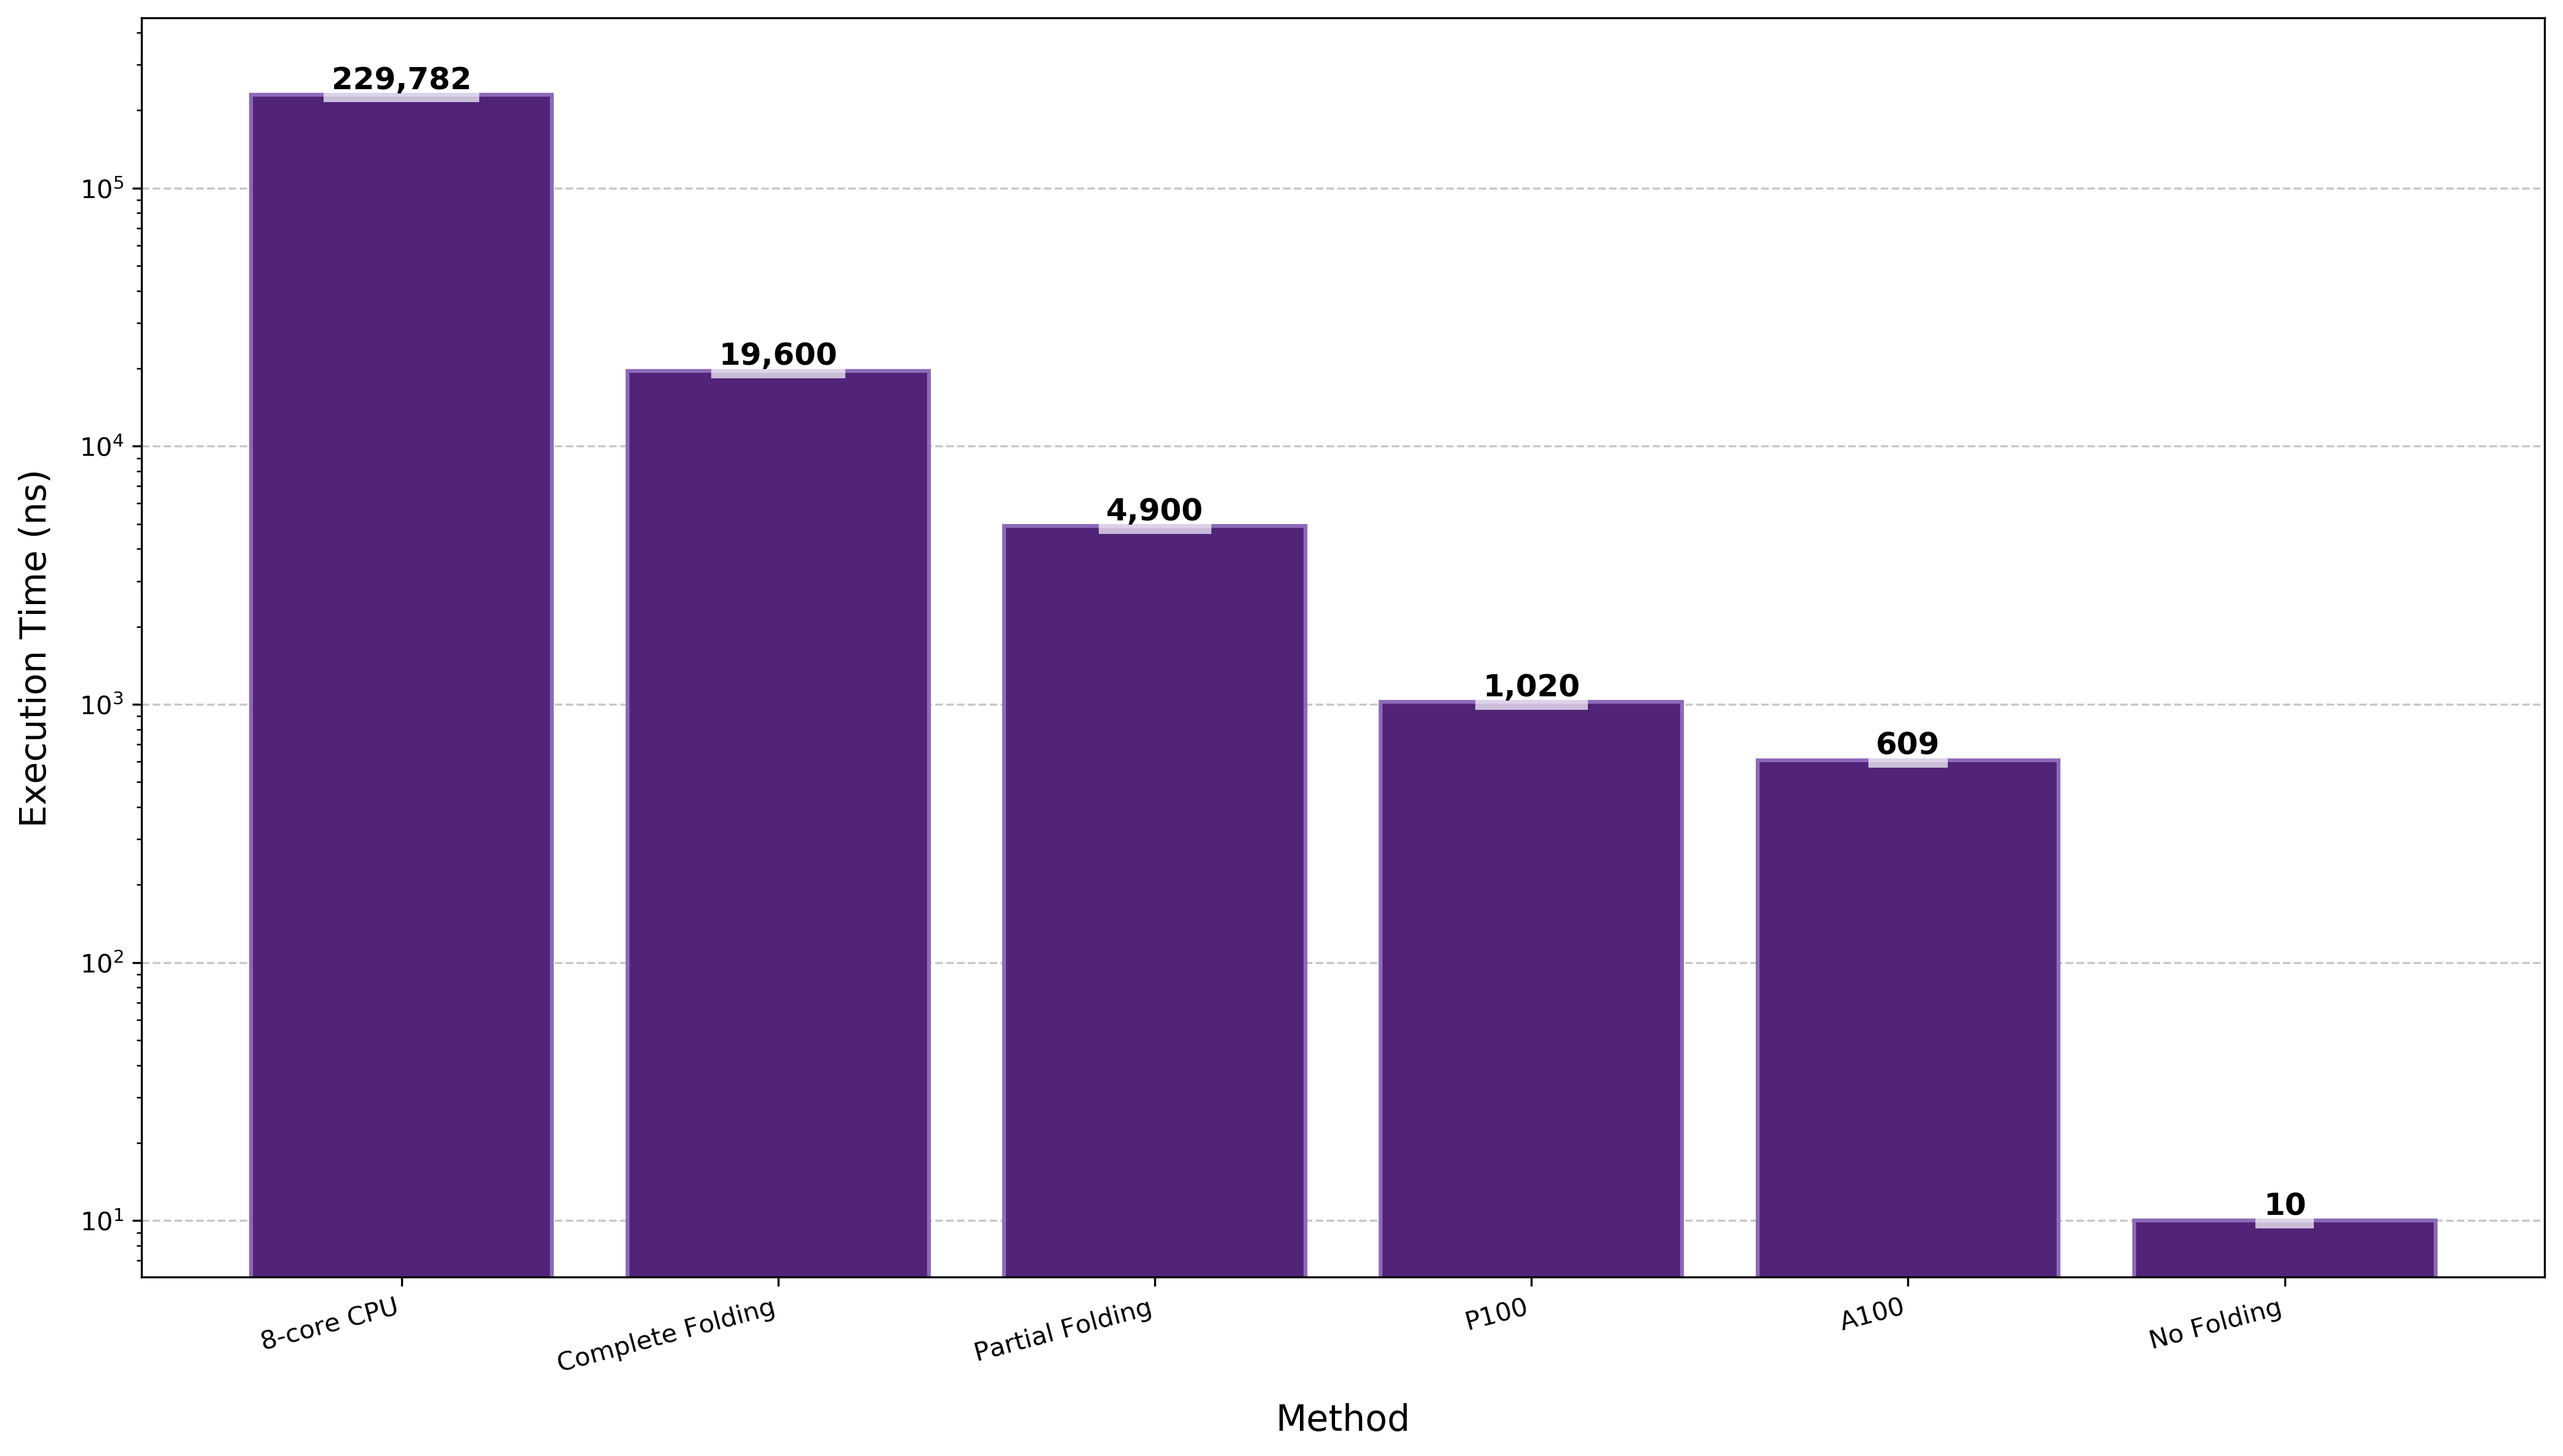
\includegraphics[width=0.75\textwidth]{chart_ex_time.png}
    \caption{Logarithmic scale of the latency of the design against the CPU and GPUs selected.}
    \label{fig:throughput_comparison}
\end{figure}
These results demonstrate that while FPGAs cannot match the absolute performance of modern GPUs for convolution operations, they offer significant advantages over CPU implementations while maintaining lower power consumption and cost compared to GPU solutions. This positions FPGA implementations as particularly suitable for embedded and edge computing applications where power efficiency and cost are primary concerns.

\clearpage
\section{Accuracy}
Hardware implementations of convolution operations must balance resource utilisation against computational precision. Enable time multiplexing (referred to as folding) is used to separate the input image over different time intervals to reduce the number of MAC units required for processing. While this approach effectively reduces hardware resource consumption, it introduces potential sources of computational error not present in software implementations.

At a hardware layer, the accuracy between software and hardware implementations can vary due to several factors:
\begin{itemize}
    \item The precision of the data types used in the design
    \item The potential for overflow or underflow in arithmetic operations
    \item The accumulation of rounding errors in sequential computations
\end{itemize}

\begin{figure}[h]
    \centering
    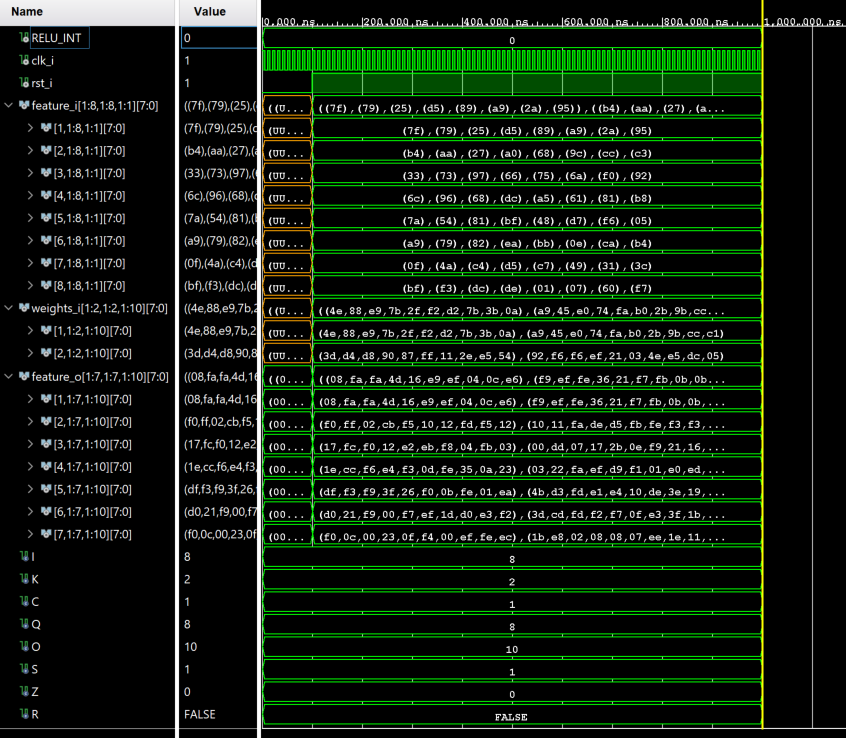
\includegraphics[width=0.9\textwidth]{tb_conv.png}
    \caption{Simulation waveform demonstrating fully parallelised implementation timing.}
    \label{fig:sim_parallel}
\end{figure}

To validate the accuracy of the design, a pseudo-random generator is used to prevent bias in the image and the weights. A testbench is then employed to simulate the operation of the design, and compare the output against the expected result using a software-based implementation for verification.

Figure \ref{fig:sim_parallel} provides a simulation waveform demonstrating the timing of the fully parallel implementation. When the setup time is complete, the output is available on the next clock cycle. This implementation requires minimal control logic, with its behavior primarily determined by the number of MAC units and the kernel size. As expected, the fully parallel implementation achieves the highest accuracy, completing operations in a single clock cycle with no detectable error when compared against the software reference.

The partially folded and folded implementations share the same approach for handling the dataflow component. However, analysis reveals a single error in one MAC operation present in both folding designs. While this introduces a small deviation from the expected results, the timing characteristics remain unaffected, with operations completing in the expected number of clock cycles. Figure \ref{fig:sim_partial} shows the simulation waveform for the partially folded implementation, demonstrating the trade-off between resource utilisation and computational precision.

\begin{figure}[h]
    \centering
    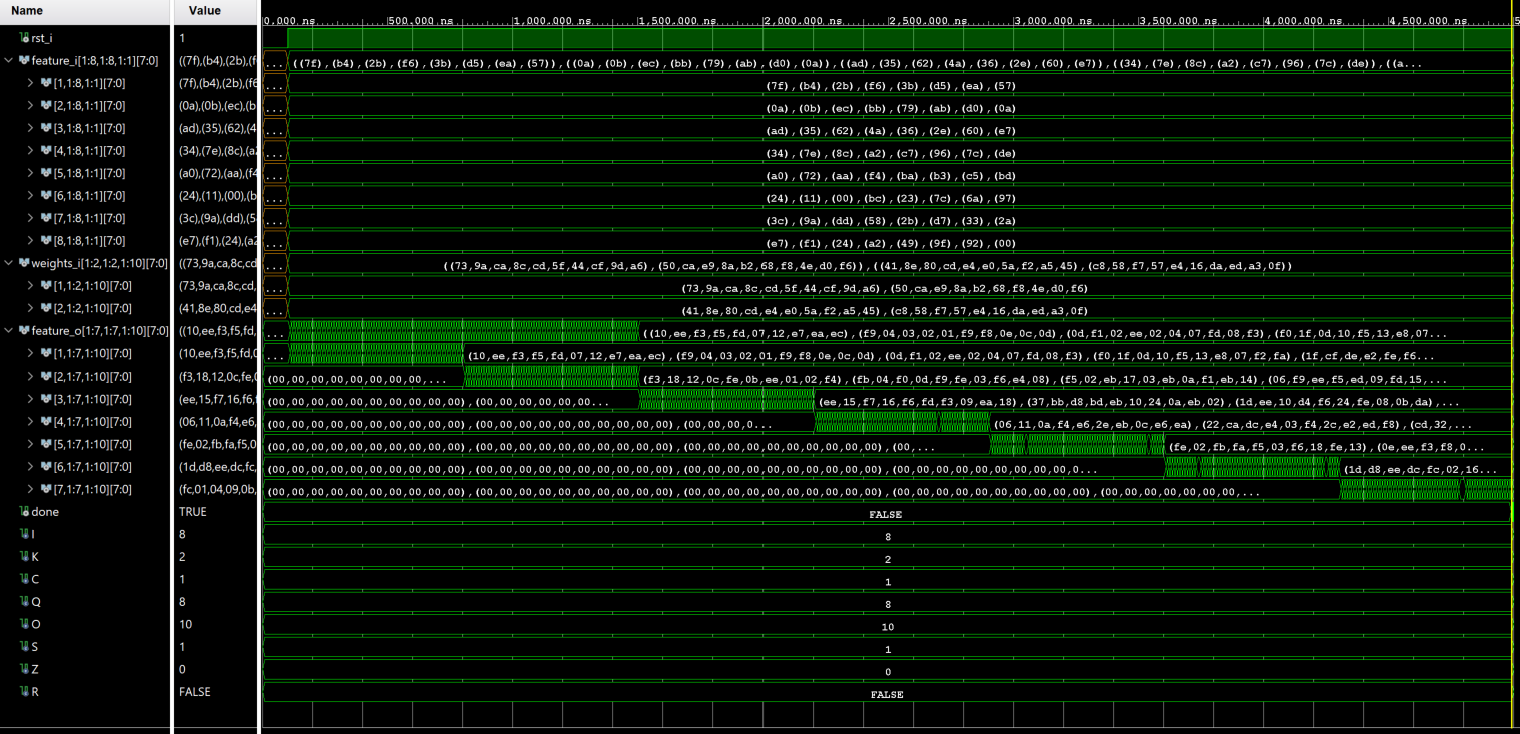
\includegraphics[width=0.9\textwidth]{tb_conv_folded.png}
    \caption{Simulation waveform demonstrating partially folded implementation timing.}
    \label{fig:sim_partial}
\end{figure}

\section{Resource Utilisation}
Resource utilisation is an integral part in validating the feasibility of implementing the design on a particular FPGA or microchip, due to the limited resources available. The three implementation approaches demonstrate distinct trade-offs between parallelization and hardware requirements, each suited to different application constraints.

\subsection{Hardware Requirements}
The number of hardware multipliers and adders required for each implementation are deterministic, similar to that of the clock cycles required.
This directly translates to the number of LUTs required for the design.

For the sequential MAC of the fully parallelised implementation, the number of multipliers is dependent on the kernel size as this determines the number of operations required.

\begin{equation}
    M_{fully\ parallel} = K^2 \times C \times O
\end{equation}

The adders will be one less than the number of multipliers, as the final operation does not require an adder.

\begin{equation}
    A_{fully\ parallel} = M_{fully\ parallel} - 1
\end{equation}

For the partially folded implementation, the adders and multipliers are shared across time. 
This allows for an independency from the number of output channels, as the number of operations is fixed by the kernel size.

\begin{equation}
    M_{partially\ folded} = K^2
\end{equation}

\begin{equation}
    A_{partially\ folded} = K^2 - 1
\end{equation}

A fully folded implementation will only require a single MAC unit, as all operations are performed sequentially. Hence, a constant number of both adders and multipliers are required with a value of 1 - independent of the kernel size.
\begin{equation}
    M_{fully\ folded} = 1
\end{equation}

\begin{equation}
    A_{fully\ folded} = 1
\end{equation}

\subsection{Implementation}
The resource utilisation across implementations demonstrates the trade-offs between parallelization and FPGA resource consumption. Table \ref{tab:resource_comparison} shows the percentage utilisation of key FPGA resources for each design variant.

\begin{table}[h!]
    \centering
    \caption{Resource utilisation comparison of convolutional core implementations}
    \label{tab:resource_comparison}
    \begin{tabular}{lcccc}
        \toprule
        Implementation & LUTs & Registers & F7 Muxes & F8 Muxes \\
        \midrule
        No Folding & 144061 (692.60\%) & 3430 (8.25\%) & 0 (0\%) & 0 (0\%) \\
        Partially Folded & 1622 (7.8\%) & 3456 (8.31\%) & 0 (0\%) & 0 (0\%) \\
        Fully Folded & 2551 (12.26\%) & 9511 (23.10\%) & 592 (3.63\%) & 240 (2.94\%) \\
        \bottomrule
    \end{tabular}
\end{table}

The no-folding implementation represents a fully parallelized approach, where all operations are performed simultaneously. While this achieves optimal performance, the resource requirements (692.60\% of available LUTs) make it impractical for implementation on most FPGAs. This demonstrates the fundamental limitation of full parallelization: the hardware requirements scale linearly with the size of the convolution operation.

The partially folded implementation introduces time multiplexing through dataflow control logic, significantly reducing hardware requirements to just 7.8\% of available LUTs. This dramatic reduction comes with minimal overhead in control logic, representing an efficient compromise between resource utilisation and performance.

Interestingly, the fully folded implementation, despite using only a single MAC unit, shows higher resource utilisation (12.26\% LUTs) than the partially folded approach. This counter-intuitive result stems from the complex control logic required to manage the sequential processing of operations. The additional registers (23.10\%) and multiplexers (F7: 3.63\%, F8: 2.94\%) needed for control flow management effectively negate the resource savings from reduced MAC units.

These results demonstrate that aggressive resource optimization through full folding may not always yield the most efficient implementation. The partially folded architecture achieves a better balance, significantly reducing resource requirements while maintaining manageable control complexity.

\section{Efficiency}
As noted, the produced hardware designs are markedly slower than the GPU implementations.
However, this is not an even comparison, due to the differing hardware resources available.
Hence, it is more effective to provide the metric for the convolutional cores using an efficiency metric instead of pure throughput.
To quantify implementation efficiency, we define a metric that relates performance to resource utilisation.

\begin{equation}
    \text{Efficiency} = \frac{\text{Throughput (images/s)}}{\text{LUT Utilization (\%)}}
\end{equation}

\begin{table}[h!]
    \centering
    \caption{Efficiency comparison of convolutional core implementations}
    \label{tab:efficiency_comparison}
    \begin{tabular}{lcccc}
        \toprule
        Implementation & Efficiency \\
        \midrule
        No Folding & 10e8 \\
        Partially Folded & 26153.8 \\
        Fully Folded & 4159.9 \\
        \bottomrule
    \end{tabular}
\end{table}


This metric reveals that the partially folded implementation achieves an efficiency of 26,153.8, significantly outperforming the fully folded design's efficiency of 4,159.9. This substantial difference in efficiency (6.29x) demonstrates that the partially folded architecture strikes an optimal balance between resource utilisation and performance for the target application.

While GPU implementations achieve superior absolute throughput, with the Tesla P100 processing 9.8e6 images/second, they represent a fundamentally different point in the design space, optimized for high-performance computing rather than embedded applications. The partially folded FPGA implementation offers a more appropriate solution for resource-constrained environments, providing a 46.9x speedup over CPU implementation while maintaining modest resource requirements.

These results demonstrate that the relationship between folding factor and implementation efficiency is non-linear, with the partially folded architecture representing a local optimum in the design space. This finding has significant implications for future FPGA-based CNN accelerator designs, suggesting that moderate levels of resource sharing can achieve better overall system efficiency than either extreme of the folding spectrum.

\section{RISC-V processor}
The NeoRV32 processor consumed little of the hardware resources, as it effectively acts as a method to memory map a peripheral such that the convolution or machine learning cores can access the location of an input image.
Communication is implemented with a 32-bit wide wishbone interface, and a buffer used to ingest the data to the core.
The usage of the RISC-V processor is provided in table \ref{tab:riscv_usage}.

\begin{table}[h!]
    \centering
    \caption{Usage of the RISC-V processor}
    \label{tab:riscv_usage}
    \begin{tabular}{lccc}
        \toprule
        Resource & Used & Available & Utilization (\%) \\
        \midrule
        LUTs & 1934 & 20800 & 9.30\% \\
        Registers & 1350 & 41600 & 3.25\% \\
        F7 Muxes & 1 & 16300 & 0.006\% \\
        F8 Muxes & 0 & 8150 & 0\% \\
        \bottomrule
    \end{tabular}
\end{table}

Equally, the processor can interface via a memory mapped interface to the convolutional cores.
Common designs employ camera modules directly on the FPGA, which require BRAM to store the incoming image data.
This can be used to abstract away from the use of a 32-bit wide wishbone interface, and instead use a memory mapped interface to the convolutional cores.
The NeoRV32 processor can then be used as a controller to start the convolution operation, and to retrieve the output signal. 

\section{Quantisation}
The quantisation of the weights allows for truncating of the number of bits used to represent the weights, which in turn reduces the resources required for implementing the convolution operation. As demonstrated in the design phase, for the given neural network, this is a mostly lossless operation, with a negligible impact on the accuracy of the network.

The effectiveness can be computed based on the utilisation of the FPGA resources when compared to the baseline design. The model was reconstructed using 2, 4, 8 and 16 bit precision weights to compare the utilisation of the FPGA resources on the unfolded convolution core.

\begin{table}[h]
    \centering
    \caption{Utilisation of the FPGA resources when compared to the baseline design.}
    \label{tab:quantisation_utilisation}
    \begin{tabular}{lcccc}
        \toprule
        Bit Quantisation & LUTs & Registers \\
        \midrule
        2-bit & 11033 (53.04\%) & 980 (2.36\%) \\
        4-bit & 44591 (214.38\%) & 1960 (4.71\%) \\
        8-bit & 144061 (692.60\%) & 3430 (8.25\%) \\
        16-bit & 570540 (2742.98\%) & 7510 (18.05\%) \\
        \bottomrule
    \end{tabular}
\end{table}

The results demonstrate significant resource savings through weight quantisation. Reducing precision from 16-bit to 8-bit yields a 4x reduction in LUT utilisation (from 2742.98\% to 692.60\%). Further reduction to 4-bit provides an additional 3.2x improvement, while 2-bit quantisation achieves a 13x reduction compared to the 8-bit baseline.

This dramatic reduction in resource utilisation is achieved by performing quantisation during the training phase, where the network learns to operate with reduced precision weights. The hardware implementation then benefits from these smaller bit widths without requiring additional computation for runtime quantisation.

In hardware, these quantised operations can be efficiently implemented through bit shifting operations. For example, multiplication by powers of 2 can be achieved through left shifts, while division can be implemented through right shifts. This approach eliminates the need for complex floating-point arithmetic units, further reducing hardware complexity and improving performance. The general form for this operation can be expressed as:

\begin{equation}
    result = input \ll n
\end{equation}

Where $n$ represents the number of bit positions to shift, and $\ll$ denotes a left shift operation.

The trade-off between precision and resource utilisation becomes particularly apparent when examining the register usage. While LUT consumption scales exponentially with bit width, register utilisation shows a more linear relationship, suggesting that control logic overhead remains relatively constant across different quantisation levels.

These findings indicate that aggressive quantisation (2-bit or 4-bit) can make otherwise impractical designs feasible on resource-constrained FPGAs, provided the application can tolerate the associated reduction in numerical precision. For many neural network inference tasks, this trade-off is acceptable, as modern training techniques can compensate for reduced precision through appropriate weight adjustment during the training phase.
This is the basis of binarized neural networks, which provide a single-bit precision to substantially compress the neural network at the training level \cite{18}.

\section{Extensibility}
The project aims to provide a flexible design that can be extended to support other machine learning algorithms. While the core components of neural networks - convolution, pooling, and fully connected layers - all fundamentally rely on MAC operations, their direct implementation often exceeds available FPGA resources. This section explores the practical considerations and solutions for implementing these components on resource-constrained hardware.

\subsection{Resource Constraints}
Without folding techniques, the implementation of a complete neural network becomes impractical on most FPGAs. This is particularly evident in fully connected layers, which require a MAC unit for each input-weight combination. For example, a fully connected layer with 1024 inputs and 10 outputs would require 10,240 MAC units - far exceeding the resources of typical FPGAs.

The solution lies in applying appropriate folding strategies to each layer type:
\begin{itemize}
    \item Convolution layers can utilize partial folding to balance parallelism and resource usage
    \item Pooling operations can share MAC units through time multiplexing
    \item Fully connected layers require aggressive folding due to their dense computation requirements
\end{itemize}

\subsection{Implementation Architecture}
The described machine learning core was synthesised and implemented on the Digilent Basys 3 board, employing a RISC-V softcore processor to interface with the FPGA fabric. This allows for the design to be easily extended to support other machine learning algorithms, by utilising the same interface.

The testbench for this is illustrated in figure \ref{fig:tb_extensibility}. There is a significant initial setup time required to load the weights and biases into the memory, and to configure the machine learning core. However, this is a one-time operation, and only requires the RISC-V processor to be programmed. Once this is complete, the machine learning core can be used to process data streams in a time-multiplexed manner, with no additional overheads. This simulates effectively a cold-start of the machine learning core, which software implementations will also initially face.

\begin{figure}[h]
    \centering
    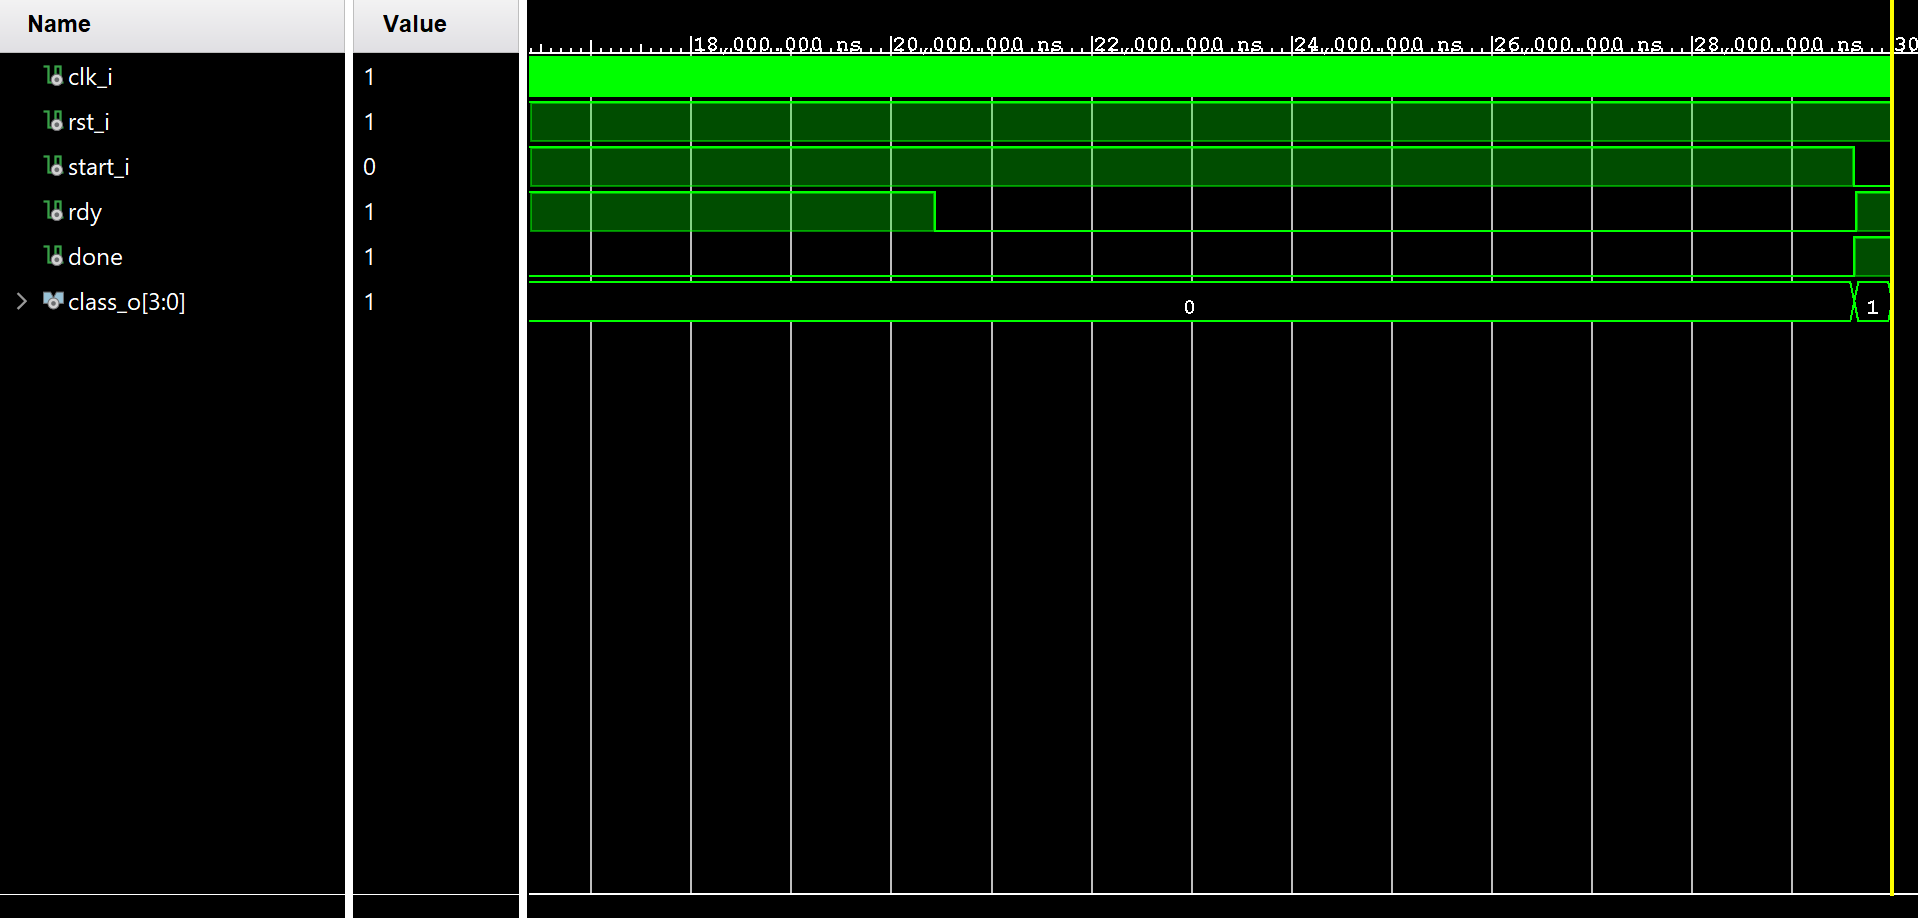
\includegraphics[width=0.9\textwidth]{tb_mem_accel.png}
    \caption{Simulation waveform demonstrating the extensibility of the design.}
    \label{fig:tb_extensibility}
\end{figure}

\subsection{Resource Sharing}
The key to implementing complex neural networks on FPGAs lies in the strategic sharing of MAC units across different layer types. By recognizing that convolution, pooling, and fully connected layers all fundamentally perform multiply-accumulate operations, a unified hardware architecture can be designed that time-multiplexes these resources effectively.

This approach offers several advantages:
\begin{itemize}
    \item Reduced resource utilization through hardware reuse
    \item Simplified control logic through standardized interfaces
    \item Flexibility to implement different network architectures
    \item Scalability to accommodate larger networks within resource constraints
\end{itemize}

The trade-off between performance and resource utilization can be dynamically adjusted through the folding factor, allowing the same design to be adapted for FPGAs with different resource constraints. This flexibility makes the architecture suitable for a wide range of applications, from edge computing devices to more capable FPGA platforms.


% HOW TO ADD ADDITIONAL CHAPTERS
% Step One: Add a new folder called "ChapterX" (X being the chapter number).
% Step Two: Within the folder add a new .tex file by clicking the "New File" button in the Overleaf Menu. Rename the file to a title of your choice.
% Step Three: Copy the Chapter 2 headline and "\input" command located above and insert it below Chapter 2.
% Step Four: Rename the headline to your specific chapter number, change the input command to include the name of the folder you created and the name of the file you created.
% Repeat this process for every chapter.

%CONCLUSION CHAPTER
\chapter[Conclusion]{Conclusion}
\label{Chap:Conclusion}

This chapter summarizes the key findings and contributions of this thesis, discussing both the achievements and limitations of the hardware-based CNN implementation. Additionally, it outlines potential future work and recommendations for extending the design.

\section{Summary}

The research demonstrates the viability of hardware-accelerated convolution operations for resource-constrained embedded systems. Through the implementation and analysis of three distinct approaches to hardware convolution, this thesis has shown that effective trade-offs between parallelization and resource utilization are crucial for practical FPGA-based CNN acceleration.

The partially folded implementation emerged as the most effective solution, offering an optimal balance between resource utilization and performance. While the fully unrolled design theoretically offers maximum throughput, FPGA resource constraints, as discussed in Section \ref{sec:platforms}, made this approach impractical for real-world deployment. The fully folded implementation, despite its minimal resource usage, introduced significant control overhead that ultimately negated its resource advantages, aligning with the findings from previous research on hardware-based CNN implementations.

The integration with the NEORV32 RISC-V processor proved particularly significant, demonstrating a practical approach to hardware acceleration in SoC designs. As explored in the literature review, RISC-V's open-source nature and extensibility make it an ideal choice for embedded systems. The processor effectively manages data flow and control operations while offloading compute-intensive tasks to dedicated hardware accelerators, creating an efficient architecture for resource-constrained environments.

\section{Key Contributions}

This thesis contributes to the field of hardware-accelerated neural networks by developing configurable, generic hardware blocks for CNN implementation. This addresses the need for flexible, resource-efficient solutions in embedded systems. The successful integration with RISC-V demonstrates a practical approach to hardware acceleration, building upon existing research in FPGA-based CNN implementations.

The analysis of resource-performance trade-offs provides valuable insights for future FPGA-based CNN acceleration projects. The implementation of parallel MAC units with configurable folding factors offers a flexible solution that can be adapted to various resource constraints, addressing a key challenge identified in the literature review regarding the balance between parallelization and resource utilization.

\section{Limitations}

The research revealed several important limitations that warrant further investigation. Resource constraints fundamentally limit the maximum achievable parallelization, a challenge consistently noted in FPGA-based CNN implementations. As image and kernel sizes increase, timing constraints become increasingly problematic, necessitating more sophisticated approaches to maintain performance.

While the performance gap compared to GPU implementations is significant, this limitation stems from the inherent resource constraints of the target environment rather than the implementation approach. As discussed in Section \ref{sec:platforms}, GPUs benefit from thousands of CUDA cores and specialized architectures for parallel processing, advantages that cannot be replicated in resource-constrained FPGA environments.

The current implementation's lack of direct camera interface integration and the need for off-chip memory to store weights for large neural networks represent practical limitations that affect real-world deployment. These challenges align with those identified in previous research on embedded CNN implementations.

\section{Future Work}

Future research should focus on several key areas to address the identified limitations while maintaining the resource-efficient approach demonstrated in this thesis. Hardware optimizations could include the development of parallel adder trees or multi-cycle paths to address timing issues with larger kernels, building upon existing research in FPGA-based convolution implementations.

The RISC-V integration offers particularly promising avenues for future development. Custom instruction set extensions for CNN operations could further optimize performance, leveraging RISC-V's extensible nature as discussed in the literature review. The development of hardware-specific compiler optimizations and efficient memory-mapped interfaces could enhance the system's overall efficiency.

System integration represents another crucial area for future work. The integration of camera modules with real-time processing capabilities would enhance the practical applicability of the system. Development of efficient weight loading mechanisms and power management features would address current limitations in handling larger neural networks and improve system efficiency.

The generic nature of the developed hardware blocks provides a strong foundation for building complete CNN systems, while the RISC-V integration demonstrates a practical approach to hardware acceleration in embedded systems. Future work should focus on addressing the identified limitations while maintaining the resource-efficient approach demonstrated in this thesis.

In conclusion, this research highlights the potential of FPGA-based CNN acceleration for embedded systems, while acknowledging the inherent limitations of resource-constrained environments. The developed architecture, particularly the integration with RISC-V, provides a practical framework for future developments in hardware-accelerated machine learning applications. The findings contribute to the growing body of research on efficient hardware implementations of neural networks and offer valuable insights for future work in this field.




% ***************************************************
% Bibliography
%****************************************************
%CHOOSE YOUR BIB STYLE AND FILE.
%We have included the following two referencing styles for you to use in your thesis. You can add an alternate style if you prefer.

%Style: apalike = this is an (Author, Year) referencing style similar to APA
%Style: elsarticle-num = this is a numbered referencing style that will display the bibliography in citation order

%To use one of the styles provided ensure the % is removed from the start of the line, and the other option is commented out with a % at the start of the line. The style elsarticle-num is active by default.

%\bibliographystyle{apalike}
\bibliographystyle{elsarticle-num}

\bibliography{./References/Bibliography}

%When you have finished your thesis we recommend that you manually fix any errors in your bibliography. 
%To do this, compile, copy the .bbl into a new .tex file and include this here after commenting out the other bibliography commands. Make corrections in that .tex file.

% ***************************************************
% Appendices
%**************************************************** 
%UNCOMMENT THIS SECTION IF YOU ARE USING APPENDICES.
%Simply adapt the same formatting used for other chapters.
\appendix
% If you need appendix in your thesis then consider the following appendix file (you can add more if you need more) otherwise you should not consider it in your main thesis.
% ***************************************************
% Appendix
% ***************************************************
\chapter{Appendix}

\section{Repository}
The repository for this project can be found at \url{https://github.com/jdw5/metr4911}.

\section{Device Information}
\label{app:device_information}

\subsection{CPU Device Specifications}
\begin{table}[h]
    \centering
    \begin{tabular}{|l|l|}
        \hline
        \textbf{Component} & \textbf{Specification} \\
        \hline
        Architecture & x86\_64 \\
        CPU Cores & 8 \\
        CPU Frequency & 3100 MHz \\
        System RAM & 90 GB Total \\
        GPU & N/A \\
        GPU Memory & N/A \\
        \hline
    \end{tabular}
    \caption{System Specifications for CPU Test Environment}
    \label{tab:cpu_specs}
\end{table}

\subsection{P100 Device Specifications}
\begin{table}[h]
    \centering
    \begin{tabular}{|l|l|}
        \hline
        \textbf{Component} & \textbf{Specification} \\
        \hline
        Architecture & x86\_64 \\
        CPU Cores & 20 (Physical) / 20 (Total) \\
        CPU Frequency & 3012.026 MHz \\
        System RAM & 251.55 GB Total \\
        GPU & Tesla P100-PCIE-16GB \\
        GPU Memory & 15.90 GB \\
        \hline
    \end{tabular}
    \caption{Device Specifications for P100 test environment}
    \label{tab:p100_specs}
\end{table}

\subsection{A100 Device Specifications}
\begin{table}[h]
    \centering
    \begin{tabular}{|l|l|}
        \hline
        \textbf{Component} & \textbf{Specification} \\
        \hline
        Architecture & x86\_64 \\
        CPU Cores & 8 \\
        CPU Frequency & 2894.562 MHz \\
        System RAM & 93.88 GB Total \\
        GPU & NVIDIA A100-PCIE-40GB \\
        GPU Memory & 39.39 GB \\
        \hline
    \end{tabular}
    \caption{Device Specifications for A100 test environment}
    \label{tab:a100_specs}
\end{table}


\section{Convolution Results}

\subsection{CPU}
\begin{table}[h]
    \centering
    \begin{tabular}{|c|c|}
        \hline
        \textbf{Test Number} & \textbf{Execution Time (ns)} \\
        \hline
        1 & 213342 \\
        2 & 223891 \\
        3 & 229782 \\
        4 & 249048 \\
        5 & 252755 \\
        \hline
    \end{tabular}
    \caption{CPU Convolution Execution Times}
    \label{tab:cpu_conv_times}
\end{table}

\textbf{Test Configuration:}
\begin{itemize}
    \item Input Size: 8 x 8 x 1
    \item Kernel Size: 2 x 2 x 1 x 10
    \item Output Feature Size: 7 x 7 x 10
    \item Resolution: 8-bit
    \item Stride Steps: 1
    \item Zero Padding: 0
\end{itemize}

\subsection{P100}
\begin{table}[h]
    \centering
    \begin{tabular}{|c|c|}
        \hline
        \textbf{Test Number} & \textbf{Execution Time (ns)} \\
        \hline
        1 & 1010.27 \\
        3 & 1016.85 \\
        3 & 1020.45 \\
        4 & 1056.34 \\
        5 & 1120.34 \\
        \hline
    \end{tabular}
    \caption{A100 Convolution Execution Times}
    \label{tab:a100_conv_times}
\end{table}

% You might want to add these statistics
\textbf{Test Configuration:}
\begin{itemize}
    \item Input Size: 8 x 8 x 1
    \item Kernel Size: 2 x 2 x 1 x 10
    \item Output Feature Size: 7 x 7 x 10
    \item Resolution: 8-bit
    \item Stride Steps: 1
    \item Zero Padding: 0
\end{itemize}

\subsection{A100}
\begin{table}[h]
    \centering
    \begin{tabular}{|c|c|}
        \hline
        \textbf{Test Number} & \textbf{Execution Time (ns)} \\
        \hline
        1 & 608.35 \\
        2 & 608.73 \\
        3 & 610.98 \\
        4 & 612.70 \\
        5 & 613.58 \\
        \hline
    \end{tabular}
    \caption{P100 Convolution Execution Times}
    \label{tab:p100_conv_times}
\end{table}

\textbf{Test Configuration:}
\begin{itemize}
    \item Input Size: 8 x 8 x 1
    \item Kernel Size: 2 x 2 x 1 x 10
    \item Output Feature Size: 7 x 7 x 10
    \item Resolution: 8-bit
    \item Stride Steps: 1
    \item Zero Padding: 0
\end{itemize}

\newpage
\section{HDL Type Primitive}
\label{app:hdl_type_primitive}

A custom hardware type primitive was created for this project. 
It represents a feature with a height, width and depth to simplify the hardware design.

\begin{lstlisting}[language=VHDL]
type feature_t is array(natural range <>, natural range <>, natural range <>) of signed;
\end{lstlisting}

\section{Schematics}
The below pages are the hardware schematics for the project.
These are provided at high resolution to allow for detailed inspection.
The first page provided is the accelerator component, which describes the linking of the generic layers.
The second schematic is the accelerator connected to block RAMs to pass the weights and bias signals. It wraps the accelerator in a block RAM interface.
The third schematic is the system on chip, which receives the input image from the NeoRV32 softcore processor. It implements the previous schematic as an IP core.

\newpage
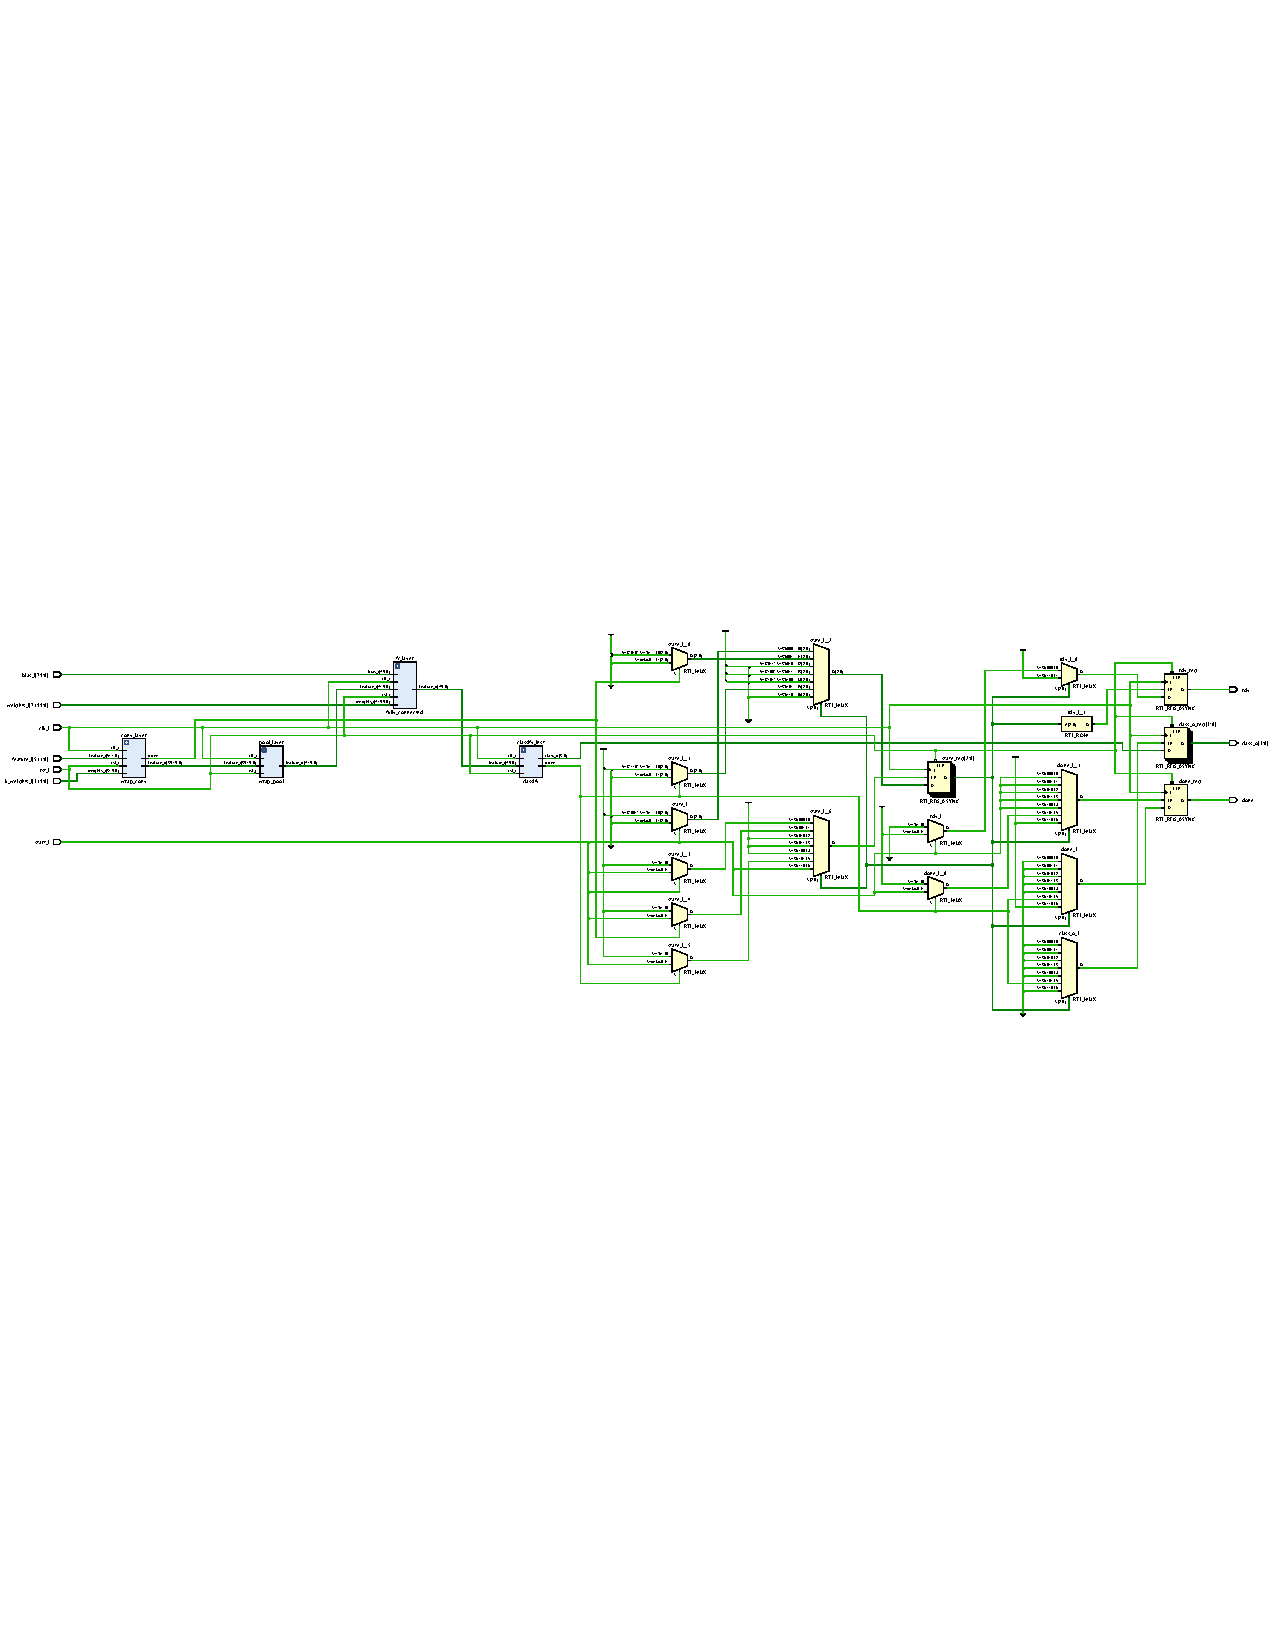
\includepdf[pages=-]{Figs/accelerator.pdf}

\newpage
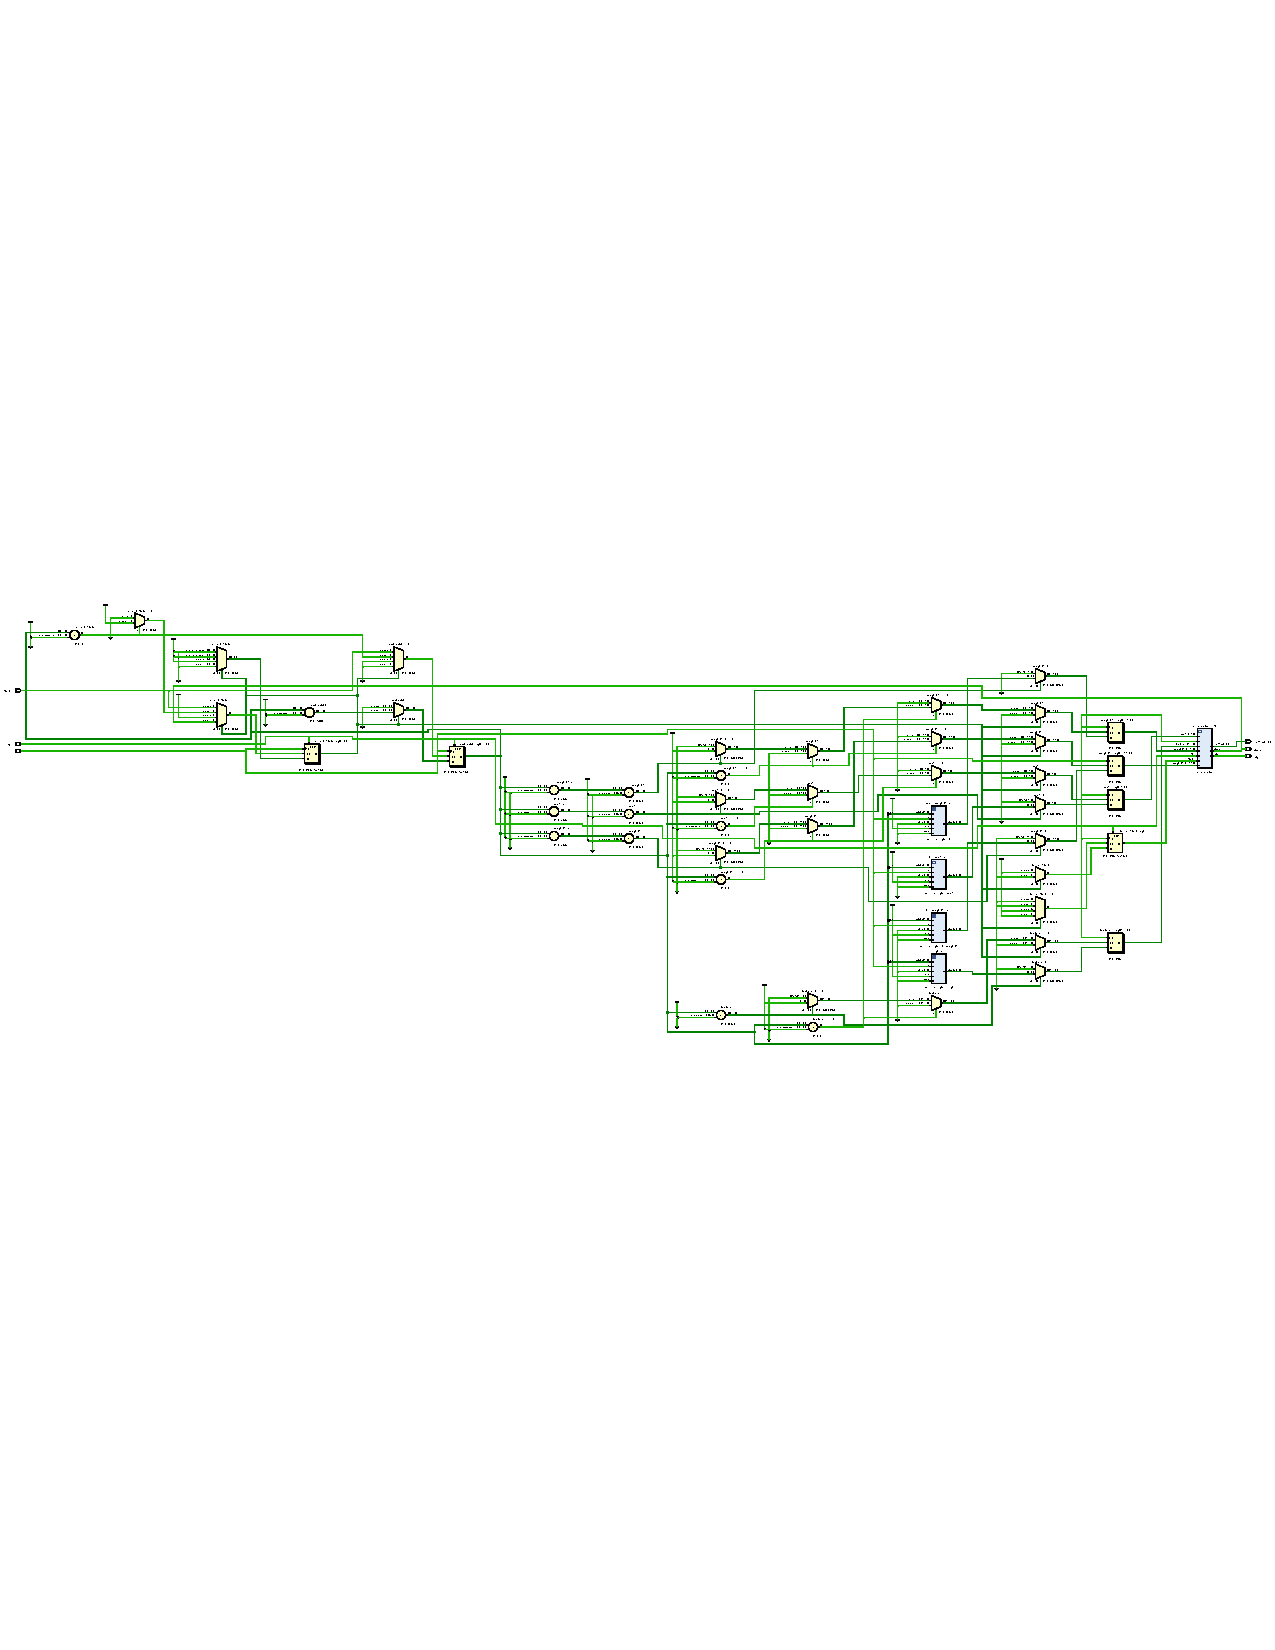
\includepdf[pages=-]{Figs/mem_accelerator.pdf}

\newpage
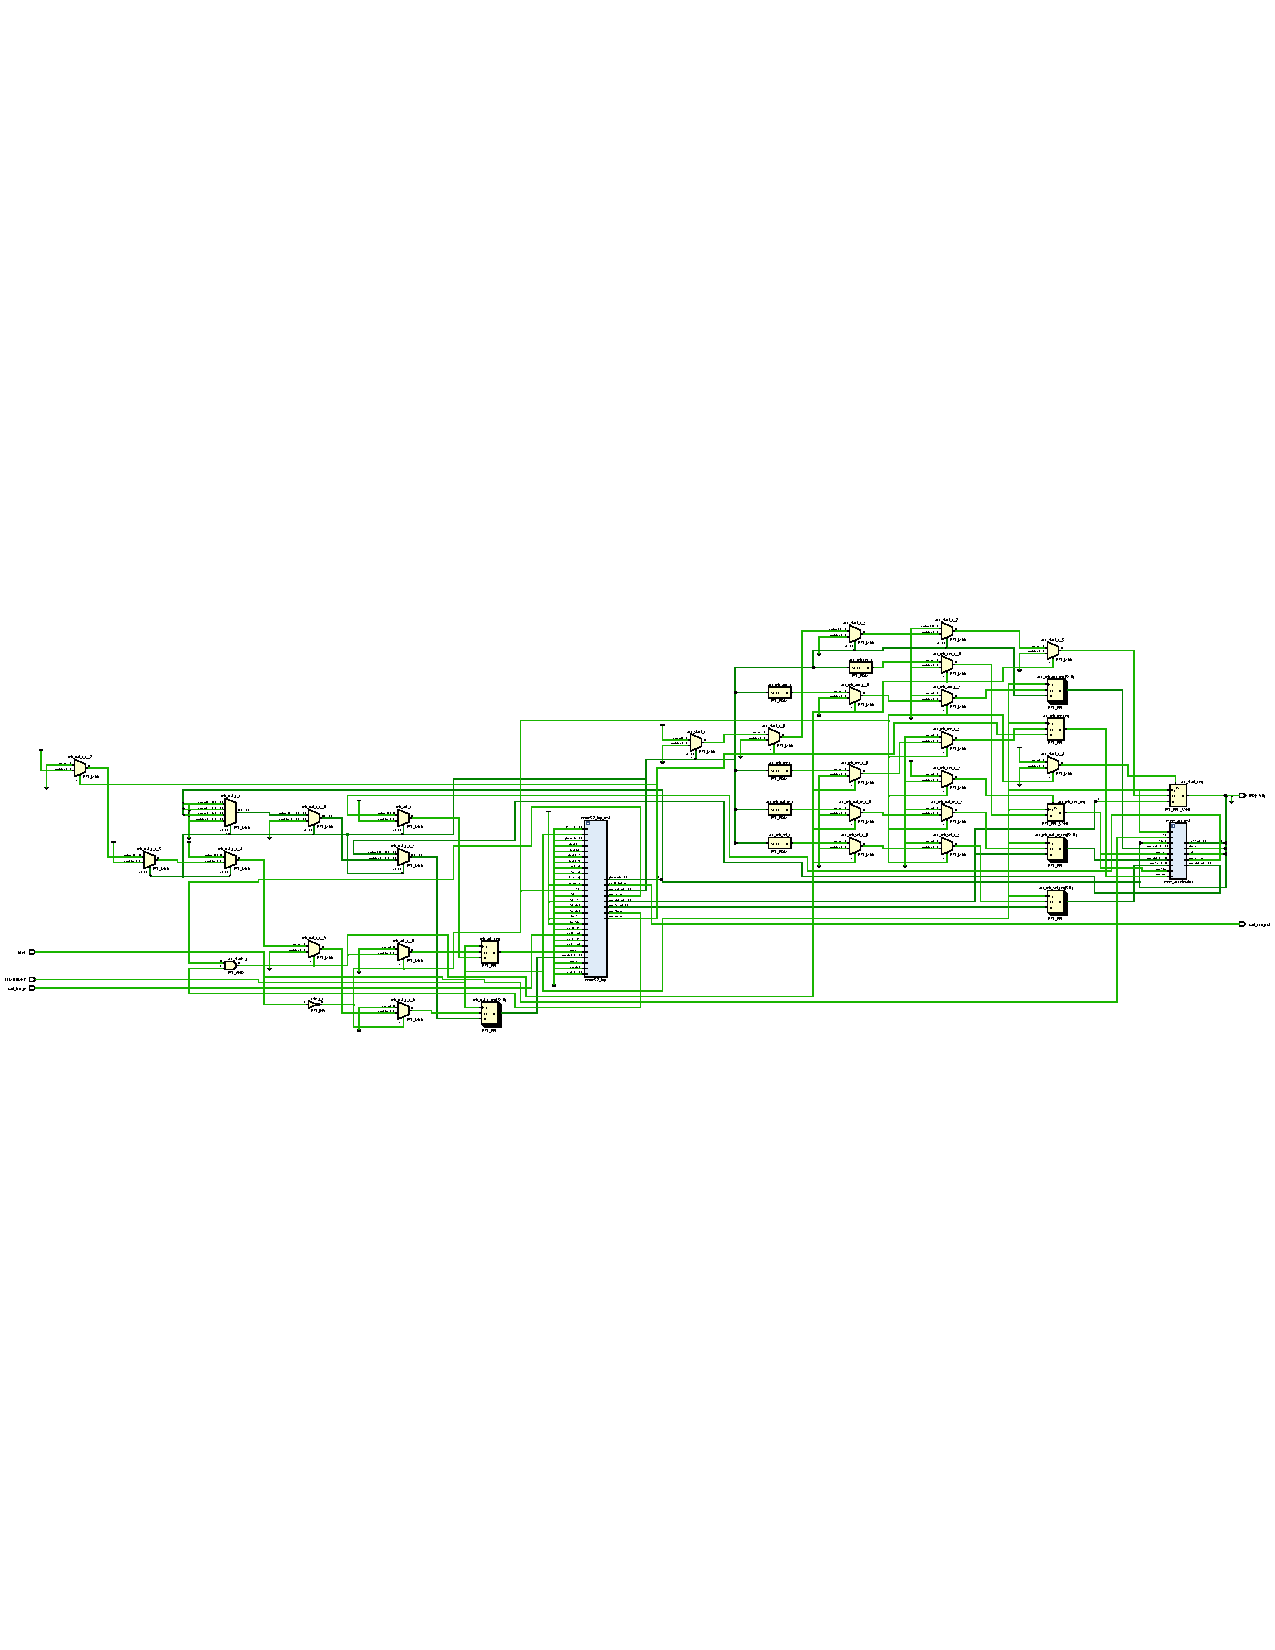
\includepdf[pages=-]{Figs/riscv-ml-core.pdf}



% ***************************************************
% Back Matter
%**************************************************** 
%COMMENT OUT IF YOU DO NOT WISH TO INCLUDE BACK MATTER.
% \input{./PreliminaryAndBackPages/Back.tex}

\end{document}
